\documentclass[11pt]{article}

% --- Geometry: ~6.5 inch text width matches matplotlib defaults in cf.viz ---
\usepackage[a4paper, margin=1in]{geometry}

% --- Math, graphics, tables ---
\usepackage{amsmath}
\usepackage{amssymb}
\usepackage{graphicx}
\usepackage{booktabs}
\usepackage{array}
\usepackage{tabularx}
\usepackage{caption}
\usepackage{subcaption}
\usepackage{microtype}

% --- Cross references ---
\usepackage[hidelinks]{hyperref}
\usepackage[noabbrev,capitalise]{cleveref}

% --- Figures live in report/figures/ ---
\graphicspath{{figures/}}

% --- Section formatting: prefix top-level headings with "Section",
%     keep subsection numbering as 1.1 / 1.2 / etc., start every
%     top-level section on a fresh page. ---
\usepackage{titlesec}
\titleformat{\section}[hang]
  {\normalfont\Large\bfseries}{Section \thesection.}{0.6em}{}
\titlespacing*{\section}{0pt}{0pt}{12pt}
\titlespacing*{\subsection}{0pt}{12pt}{6pt}

% Force every \section to start on a new page
\let\oldsection\section
\renewcommand{\section}{\clearpage\oldsection}

\begin{document}

\begin{titlepage}
    \centering
    \vspace*{2cm}

    {\Huge \textbf{Hedge Fund\\
    Panel Time Series Forecasting}}\\[1cm]

    {\Large \textbf{Course Name:} Applied Forecasting Methods}\\[2cm]

    {\Large \textbf{Group Members:}}\\[0.5cm]
    Kaushal Nandaniya (202303036)\\[0.2cm]
    Jeetraj Gohil (202303017)\\[0.2cm]
    [Member 3 Name] (Roll No: [Roll No])\\[2cm]

    {\Large \textbf{Instructor Name:} Pritam Anand}\\[2cm]

    {\Large \textbf{Institution Name:} Dhirubhai Ambani Institute of Information and Communication Technology}\\[2cm]

    {\Large \textbf{Submission Date:} \today}

    \vfill
\end{titlepage}

\begin{abstract}
This project addresses a large-scale panel time series forecasting problem derived from anonymized hedge fund data, where the objective is to predict future values of a target variable across multiple heterogeneous series under a weighted evaluation metric. The problem is challenging due to heavy-tailed distributions, extreme weight concentration, non-stationarity, and varying lengths of historical data across series.
\\
\\
The study adopts a diagnostic-driven approach, beginning with extensive exploratory data analysis to understand missingness patterns, distributional properties, and weight imbalance. Stationarity is assessed using ADF and KPSS tests, followed by transformations such as first differencing to stabilize the series. Classical forecasting models, including smoothing methods, AR, MA, ARMA, and ARIMA, are applied to representative series selected based on length, volatility, and weight characteristics. In parallel, deep learning models such as RNN, GRU, and LSTM are implemented using adaptive chronological splits to address limitations of fixed training windows.
\\
\\
The results demonstrate that no single model universally outperforms others across all series. Simple smoothing methods perform well on stable, low-variance series, while differenced ARIMA models and recurrent neural networks show superior performance on volatile and high-weight series. The findings highlight the importance of aligning model choice with data characteristics and evaluation metrics.
\\
\\
Overall, this work emphasizes that effective hedge fund forecasting requires a combination of statistical diagnostics, model adaptability, and careful consideration of panel heterogeneity.
\end{abstract}

\clearpage
\tableofcontents

\section{Problem Statement}
\label{sec:problem}

We work with a publicly released Kaggle competition dataset titled \emph{Hedge fund -- time-series forecasting}. The competition sponsor releases a panel of anonymised numerical series with engineered features and asks competitors to forecast a continuous target at four lookahead horizons. The dataset is intentionally anonymised: identifiers, feature names, and the underlying financial domain are stripped. What remains is a clean, mathematically well-defined supervised forecasting problem with a non-trivial weighting scheme.

\subsection{What is being forecast}

Each row of the panel is identified by the tuple
\[
(\mathtt{code},\ \mathtt{sub\_code},\ \mathtt{sub\_category},\ \mathtt{horizon},\ \mathtt{ts\_index})
\]
and carries a continuous target $y_{\text{target}}$, a non-negative competition weight, and 86 anonymised numerical covariates of the form $\mathtt{feature\_a}, \mathtt{feature\_b}, \ldots$ The integer time index $\mathtt{ts\_index}$ runs over the contiguous range 1--3601 in the public training partition and 3602--4376 in the held-out test partition. The training panel contains 5{,}337{,}414 rows and the test panel contains 1{,}447{,}107 rows.

The four forecast horizons are $H \in \{1,\ 3,\ 10,\ 25\}$, interpreted as the lookahead in time units. For each $(\mathtt{code},\mathtt{sub\_code},\mathtt{sub\_category})$ the panel typically carries all four horizons at the same $\mathtt{ts\_index}$, so the natural unit of analysis is the 4-tuple key above. There are 36{,}923 distinct series in train under that definition.

\subsection{Why the problem is hard}

The dataset combines three well-known difficulties that make naive baselines a bad guide:

\begin{enumerate}
  \item \textbf{Heavy-tailed target.} The target distribution is centred near zero with an interquartile range of approximately $\pm 0.05$, but the full range runs from roughly $-2200$ to $+2300$. The 1\% and 99\% percentiles are at approximately $\pm 82$. Plain mean-squared losses are therefore extremely sensitive to a small number of tail rows.
  \item \textbf{Concentrated evaluation weight.} The competition metric is sample-weighted, and the weights are extraordinarily skewed: the median weight is approximately $1.7 \times 10^{3}$ while the maximum is $1.4 \times 10^{13}$. As a result, the top one percent of rows by weight carry approximately 64\% of all evaluation mass, and the top five percent carry approximately 92\%. Any unweighted analysis can recommend the wrong model.
  \item \textbf{Limited per-series history at long horizons.} Although the panel is large in aggregate, only about 5\% of individual series cleanly cross the validation cutoff used in this work ($\mathtt{ts\_index}=2880$). Some series have as few as seven training points before the cutoff, which makes per-series classical fitting infeasible for many model families.
\end{enumerate}

\subsection{Why the problem is interesting}

Beyond being a real competitive forecasting problem, three properties make the dataset a useful subject for a methodological course project:

\begin{itemize}
  \item \emph{Anonymisation forces statistical reasoning.} Without semantic feature names we cannot fall back on domain priors. Every claim must be supported by a measurable property of the data.
  \item \emph{The weighting scheme rewards precision on rare rows.} A model that improves average behaviour while degrading on the high-weight rows can lose to a simpler model. This is a mechanically different objective from standard regression and warrants explicit study.
  \item \emph{The four horizons are coupled.} As we show in \cref{sec:cumulation}, the targets at $H \in \{3,10,25\}$ are well approximated by rolling cumulative sums of the $H=1$ process. This structure is not advertised in the dataset description and admits a modelling strategy that the midway report did not consider.
\end{itemize}

\subsection{Scope of this report}

The remainder of this report covers the diagnostic and exploratory phase of the project. \Cref{sec:targets} formalises the panel keys and the chronological constraint that any validation strategy must respect. \Cref{sec:skill} develops the official competition metric in detail, with worked numerical examples and a comparison against standard error metrics. \Cref{sec:eda} carries out a full exploratory analysis: schema sanity, missingness, target and weight distributions, stationarity diagnostics, autocorrelation structure, feature audit, and three findings about the multi-horizon structure of the panel that constrain every modelling decision in subsequent chapters of the project. Modelling chapters (classical baselines, global gradient-boosted models, the multi-horizon aggregation experiment, probabilistic forecasting, and ensembles) will be added as those notebooks land.

\input{sections/02_targets_and_series}
\section{The Weighted Skill Score}
\label{sec:skill}

The competition is decided by a single scalar: the \emph{weighted skill score}. Because the rest of the project uses this metric for every model comparison, ensemble weight, and bootstrap interval, it deserves a dedicated section. We give the formula, walk through every term, work three numerical examples, and explain why a competition organiser would pick a metric of this shape over more familiar alternatives such as RMSE, MAE, or $R^2$.

\subsection{Definition}

Given truths $y_i$, predictions $\hat y_i$, and non-negative weights $w_i$ for $i=1,\ldots,n$, the weighted skill score is
\begin{equation}
\label{eq:skill}
  \text{score}(y, \hat y; w) \;=\; \sqrt{\,1 \;-\; \mathrm{clip}_{[0,1]}\!\left( \dfrac{\sum_{i} w_i\,(y_i - \hat y_i)^2}{\sum_{i} w_i\,y_i^2} \right)\,}
\end{equation}
where $\mathrm{clip}_{[0,1]}(x) = \min(\max(x,0),1)$. The function returns 1 for a perfect prediction and 0 when the prediction is no better than the all-zero forecast.

\subsection{Term-by-term walkthrough}

\paragraph{Numerator $\sum_i w_i (y_i - \hat y_i)^2$.}
This is the weighted sum of squared residuals. It is zero when $\hat y = y$ everywhere and grows quadratically with prediction error. Because the squared error is multiplied by $w_i$, rows with larger weights contribute proportionally more to the penalty. In our panel the weight distribution is extremely concentrated, so this term is dominated by a small fraction of high-weight rows.

\paragraph{Denominator $\sum_i w_i y_i^2$.}
This is the weighted ``energy'' of the truth. It is purely a function of the data, independent of the prediction, and acts as a normaliser. Without this normaliser, two panels with very different target magnitudes (for example a high-volatility horizon and a low-volatility horizon) could not be scored on the same scale.

\paragraph{The ratio.}
The ratio
\[
R \;=\; \dfrac{\sum w_i (y_i - \hat y_i)^2}{\sum w_i y_i^2}
\]
is a weighted, non-centred ``unexplained variance'' measure. It is 0 when predictions are perfect and 1 when predictions are identically zero. It can exceed 1 when predictions are worse than zero (for example, when the prediction has the wrong sign at scale). It can in principle be unbounded above if the prediction is far from any reasonable point estimate.

\paragraph{The clip.}
$\mathrm{clip}_{[0,1]}(R)$ enforces $R \in [0,1]$. The lower bound at zero is automatic from the squares; the upper bound at 1 is the meaningful one. It says: \emph{no model that is worse than predicting zero gets credit for being even worse}. The clip stops the inside of the square root from going negative and ensures the score is always real. Operationally the clip rarely engages on competent models, but it makes the metric robust to a single catastrophic prediction.

\paragraph{The square root.}
The outer square root maps $1 - R$ from a variance-like quantity onto a correlation-like scale. A skill of $0.5$ corresponds to $R = 0.75$, that is, ``three quarters of weighted target energy is unexplained''. A skill of $0.95$ corresponds to $R = 0.0975$, ``ten percent of energy unexplained''. The square root makes mid-range skills feel as familiar as Pearson correlations rather than as compressed variance ratios.

\subsection{Worked numerical examples}

To make the behaviour of \cref{eq:skill} concrete, consider three predictions on a tiny five-row panel where the truth and weights are
\[
y = (1, 2, 3, 4, 5)^\top, \qquad w = (1, 1, 1, 1, 10)^\top.
\]
Note the heavy concentration: the last row carries 10/14 of the total weight. The weighted target energy is $\sum w_i y_i^2 = 1 + 4 + 9 + 16 + 250 = 280$.

\begin{table}[h]
\centering
\caption{Behaviour of the weighted skill score on three contrasting predictions.}
\label{tab:skill_examples}
\begin{tabular}{lrrrr}
\toprule
Prediction $\hat y$ & Numerator & Ratio $R$ & $\mathrm{clip}(R)$ & Skill \\
\midrule
$(1,2,3,4,5)$ — perfect            & $0$    & $0.000$ & $0.000$ & $1.000$ \\
$(0,0,0,0,0)$ — zero               & $280$  & $1.000$ & $1.000$ & $0.000$ \\
$(0.9,1.9,3.1,4.0,4.9)$ — close    & $0.13$ & $0.000$ & $0.000$ & $0.999$ \\
$(2,4,6,8,-5)$ — wrong sign tail   & $1014$ & $3.621$ & $1.000$ & $0.000$ \\
\bottomrule
\end{tabular}
\end{table}

A few things are worth noticing in \cref{tab:skill_examples}. First, predicting all zeros lands exactly at skill = 0, the natural reference point. Second, a prediction that is wildly wrong on the high-weight last row is clipped to skill = 0; the metric does not pay attention to how much worse than zero the model is. Third, a small-error model on the four low-weight rows but a slightly larger error on the high-weight row could already drop the skill noticeably, because the high-weight row dominates the numerator.

\subsection{Comparison against standard regression metrics}

\Cref{tab:metric_comparison} contrasts the weighted skill score with the metrics most often reported in regression problems on the same five-row toy example.

\begin{table}[h]
\centering
\caption{Behaviour of standard metrics versus the weighted skill score on the same toy panel.}
\label{tab:metric_comparison}
\begin{tabular}{lrrrr}
\toprule
Prediction $\hat y$ & RMSE & weighted RMSE & $R^2$ & Skill \\
\midrule
$(1,2,3,4,5)$           & $0.000$ & $0.000$ & $1.000$ & $1.000$ \\
$(0,0,0,0,0)$           & $3.317$ & $4.472$ & $-0.367$ & $0.000$ \\
$(0.9,1.9,3.1,4.0,4.9)$ & $0.114$ & $0.097$ & $0.999$  & $0.999$ \\
$(2,4,6,8,-5)$          & $5.200$ & $8.510$ & $-3.36$  & $0.000$ \\
\bottomrule
\end{tabular}
\end{table}

The skill score and weighted RMSE rank the four predictions in the same order, but they differ in two important ways. First, skill is bounded in $[0,1]$, which is easier to read on a competition leaderboard. Second, $R^2$ uses the centred denominator $\sum w_i (y_i - \bar y)^2$ while skill uses the non-centred denominator $\sum w_i y_i^2$; this makes skill more meaningful when the target is genuinely centred near zero (as it is in our panel) and avoids the embarrassing situation where $R^2$ goes negative for predictions worse than the constant mean.

\subsection{Why a competition organiser would design this metric}

Five properties of \cref{eq:skill} explain why a metric of this shape is sensible for a public-leaderboard hedge-fund forecasting task:

\begin{enumerate}
  \item \emph{Reference-relative}. Different series in a hedge-fund panel can have wildly different volatilities. Plain RMSE will always rank a model better on a low-volatility series than on a high-volatility series, even when the relative quality is identical. Dividing the squared error by the weighted target energy neutralises this scale effect, so a 1\% relative error on a 0.0001-scale series and a 1\% relative error on a 100-scale series contribute proportionally.
  \item \emph{Beat-the-zero baseline}. Predicting $\hat y = 0$ identically gives skill = 0. Any positive skill therefore signals ``the model has learned something''. This threshold is a more honest baseline than ``beat the naive lag-1 forecast'', which can be hard to define cleanly across heterogeneous series.
  \item \emph{Bounded $[0,1]$ via the clip and square root}. A bounded metric is leaderboard-friendly: scores compress into a familiar 0--1 range, making rankings easy to display and small differences easy to detect. The clip in particular makes the metric robust to an occasional catastrophic prediction, so competitors are not penalised disproportionately for one outlier row.
  \item \emph{Sample-weighted}. The weights let the organiser encode importance. In our panel, the weights are concentrated on a small number of rows, plausibly reflecting financial significance such as assets under management or notional traded size. A model that performs well on rows that ``matter financially'' is valued more than one that performs equally well across all rows.
  \item \emph{Interpretable on the correlation scale}. The square root puts the score on roughly the same scale as a Pearson correlation, which most readers find intuitive. Without the square root, mid-range skills would compress; with it, the values 0.3, 0.5, 0.7, 0.9 carry the rough qualitative meaning that practitioners assign to correlations.
\end{enumerate}

\subsection{Practical consequences for this project}

\Cref{eq:skill} is implemented once in the shared utility \texttt{cf.metrics.weighted\_skill\_score} and used by every later notebook for both model selection and final scoring. The function \texttt{cf.metrics.bootstrap\_skill} returns 95\% confidence intervals by row resampling; we report bootstrap intervals alongside every leaderboard number to avoid declaring winners that are within sampling noise of each other.

Two structural observations carry through to every subsequent modelling decision:

\begin{itemize}
  \item \textbf{High-weight rows decide the leaderboard.} Because approximately 64\% of weight sits in the top 1\% of rows (\cref{sec:weight_dist}), the score is essentially a measure of how well the model predicts those few rows. We must therefore train with sample weights, not just evaluate with them.
  \item \textbf{Plain RMSE will lie.} A model that improves average behaviour at the cost of a small degradation on a high-weight row can lose to a simpler model. We never report unweighted RMSE as a primary headline number.
\end{itemize}

\section{Dataset and Exploratory Analysis}
\label{sec:eda}

This section reports the exploratory analysis of the panel before any modelling. The aim is twofold. First, to establish the basic statistical shape of the data so that later modelling choices can be motivated rather than guessed. Second, to surface three structural findings about the panel --- multi-horizon coupling, the cumulation hypothesis, and per-horizon weight dominance --- that the midway report did not document but that materially change the modelling space. All numerical results below are produced by notebook \texttt{00\_data\_structure.ipynb} and the corresponding figures are saved as both PNG and PDF assets.

\subsection{Schema, panel scale, and train--test comparability}
\label{sec:eda:schema}

The training panel contains 5{,}337{,}414 rows, organised by 23 distinct \texttt{code} values, 180 distinct \texttt{sub\_code} values, and 5 \texttt{sub\_category} values across 4 horizons. The integer time index $\mathtt{ts\_index}$ runs over the contiguous range $[1, 3601]$. The test partition continues from $\mathtt{ts\_index} = 3602$ to 4376 with 1{,}447{,}107 rows, so test is a strict temporal suffix of train. Treating the 4-tuple $(\mathtt{code},\mathtt{sub\_code},\mathtt{sub\_category},\mathtt{horizon})$ as the natural series identifier yields 36{,}923 distinct series.

The only columns present in train but not in test are $y_{\text{target}}$ and $\mathtt{weight}$, as expected. Every category level seen in test exists in train, so there is no cold-start schema issue. The sub-code support narrows from 180 in train to 47 in test --- a coverage shift rather than a schema mismatch.

\subsection{Missing values}
\label{sec:eda:missing}

Missingness is computed on a 500{,}000-row stratified sample to keep memory in check. Of the 86 anonymised features, 48 contain at least one missing value, but the maximum missing rate across all columns is approximately 12.5\%. \Cref{fig:missingness} shows the top fifteen offenders.

\begin{figure}[h]
\centering
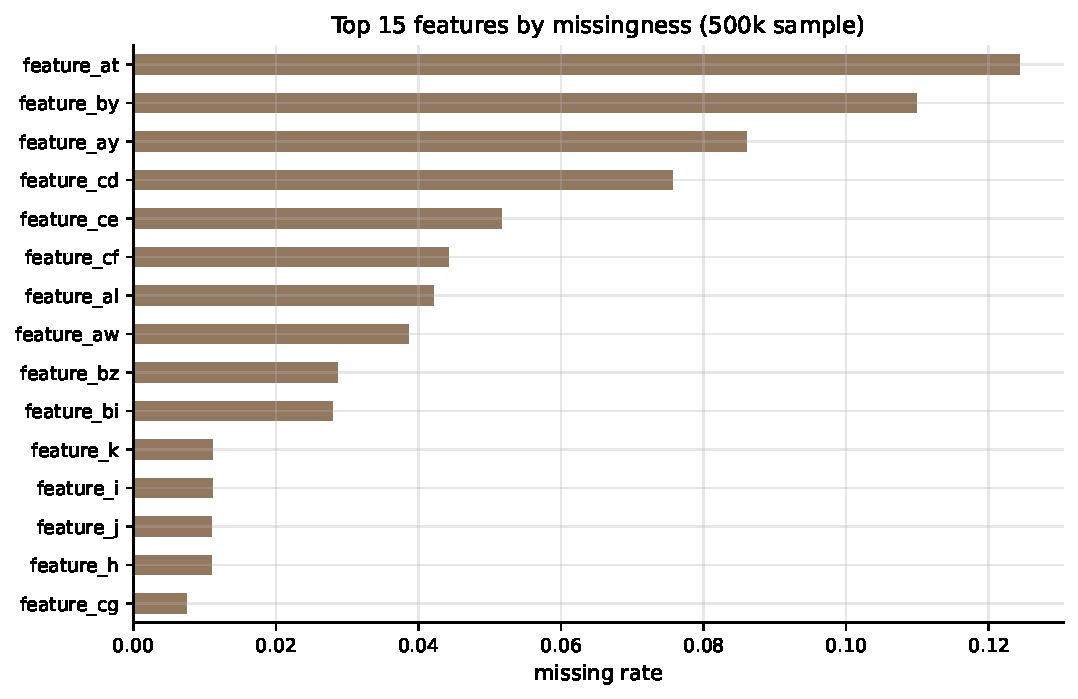
\includegraphics[width=0.85\linewidth]{00_missingness_top15}
\caption{Top fifteen features by missingness, on a 500{,}000-row stratified sample of train. The maximum missing rate is approximately 12.5\%, low enough that median imputation inside a fold is sufficient and there is no need to drop columns or use complex imputers.}
\label{fig:missingness}
\end{figure}

\paragraph{Reading.} Missing rates are bounded; within-fold median imputation suffices. No separate imputation strategy is developed.

\subsection{Target distribution}
\label{sec:eda:target}

The target $y_{\text{target}}$ is centred very close to zero (median $-0.0006$, IQR $\pm 0.05$), but has extremely heavy tails. The 1\% and 99\% quantiles sit at approximately $-82.8$ and $+62.9$ respectively, while the full range runs from approximately $-2202$ to $+2314$.

\begin{figure}[h]
\centering
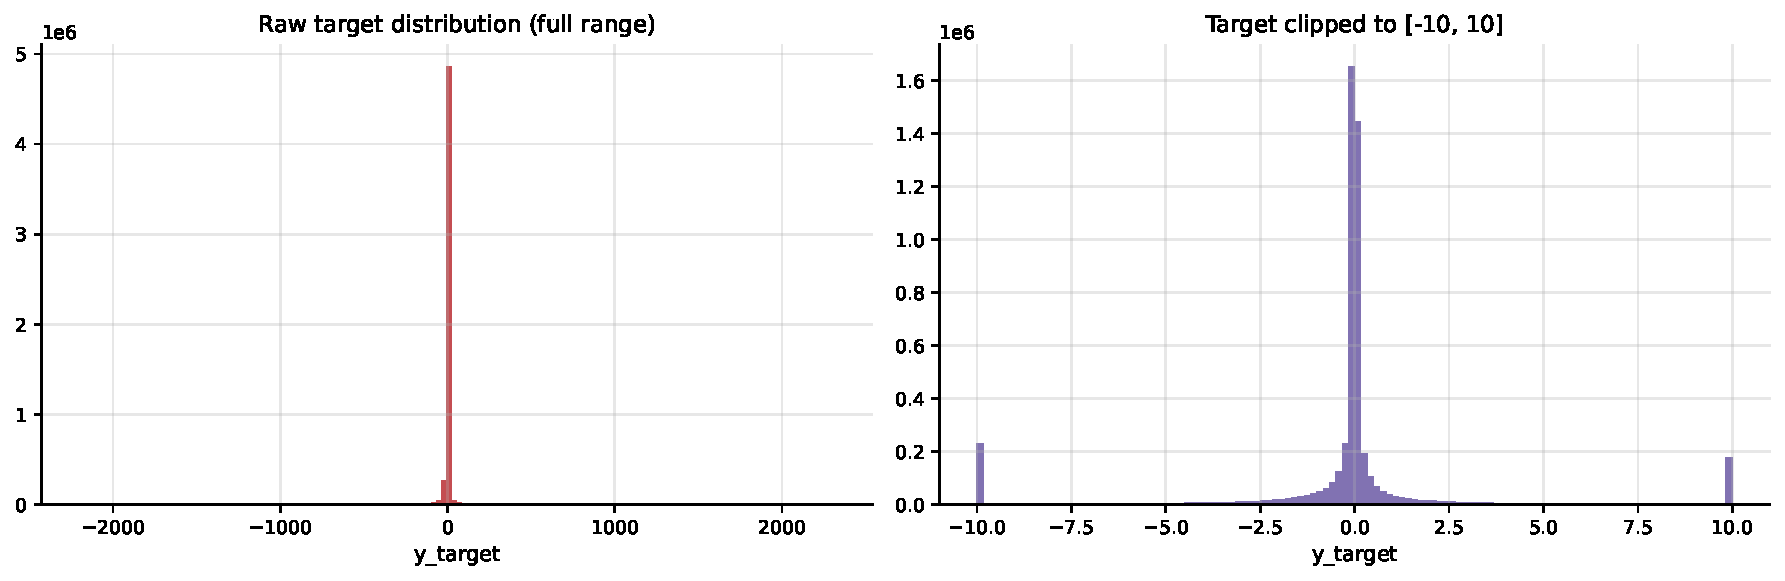
\includegraphics[width=0.95\linewidth]{00_target_distribution}
\caption{Raw target distribution (left) and the same distribution clipped to $[-10, 10]$ (right). Most of the mass concentrates near zero, with rare extreme tails up to the order of $\pm 2200$.}
\label{fig:target_dist}
\end{figure}

\paragraph{Reading.} The shape disqualifies plain unweighted MSE as a sensible loss. Tails are real outcomes, not corruption, so we cannot simply clip them; combined with the weighting scheme below, this is the central methodological constraint.

\subsection{Weight distribution and metric concentration}
\label{sec:weight_dist}

The competition weights are extraordinarily skewed. The median weight is $1{,}699$, while the maximum is $1.39 \times 10^{13}$. \Cref{fig:weight_dist} shows the weight distribution clipped at the 99th percentile (left) and the cumulative-share Lorenz-style curve (right). The top 1\% of rows carry 64.2\% of total weight; the top 5\% carry 92.6\%; the top 10\% carry 98.3\%.

\begin{figure}[h]
\centering
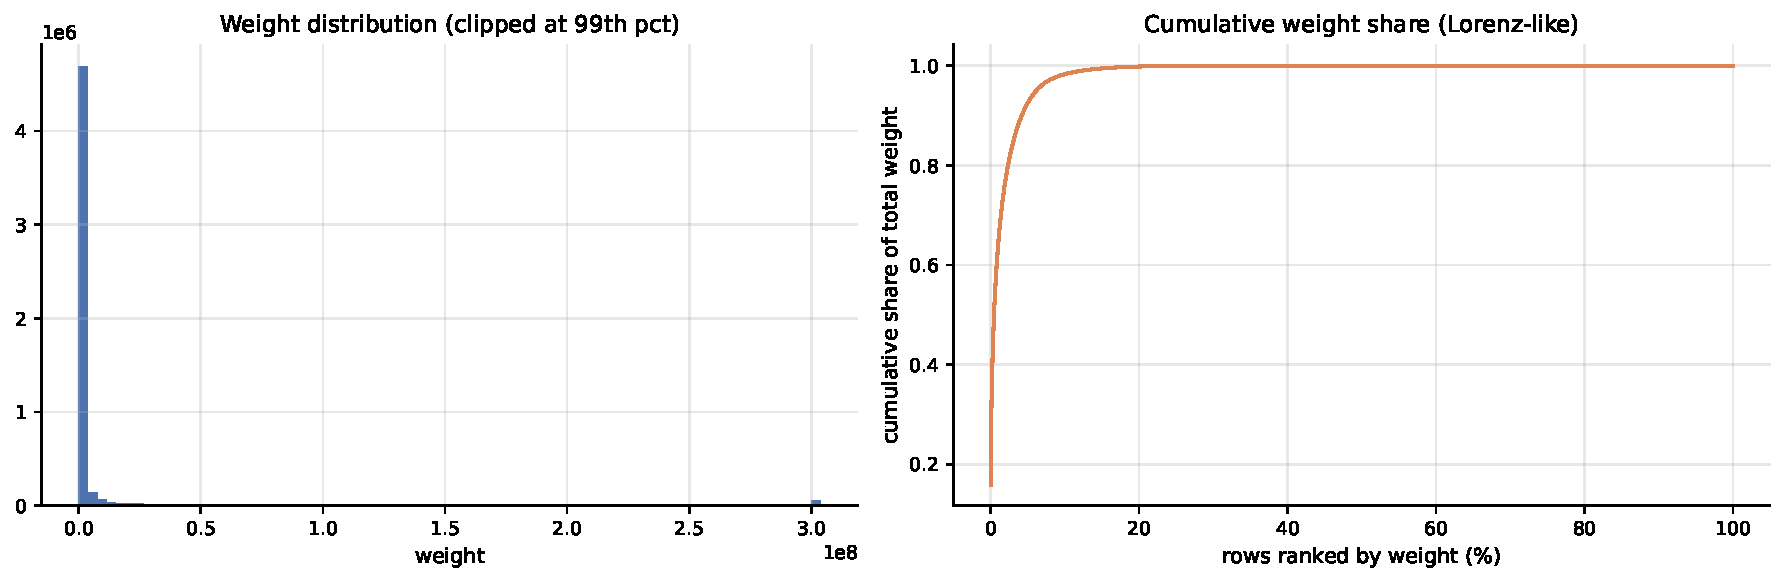
\includegraphics[width=0.95\linewidth]{00_weight_distribution}
\caption{Weight distribution clipped at the 99th percentile (left) and cumulative share of total weight ranked by weight (right). Approximately 64\% of total weight is concentrated in the top 1\% of rows; 92\% in the top 5\%.}
\label{fig:weight_dist}
\end{figure}

\paragraph{Reading.} Unweighted evaluation describes a different competition. The weighted skill score (\cref{sec:skill}) is our only headline metric, and a model that accurately predicts the top one percent of rows has more leverage on the leaderboard than a uniformly mediocre one.

\subsection{Series coverage and split feasibility}
\label{sec:eda:coverage}

Not every series has enough history to support time-based validation. \Cref{fig:series_length} shows the distribution of per-series lengths. Out of 36{,}923 distinct series, only 1{,}930 (approximately 5\%) cleanly cross the train/validation cutoff at $\mathtt{ts\_index} = 2880$. Many series end before the cutoff, contributing zero validation rows.

\begin{figure}[h]
\centering
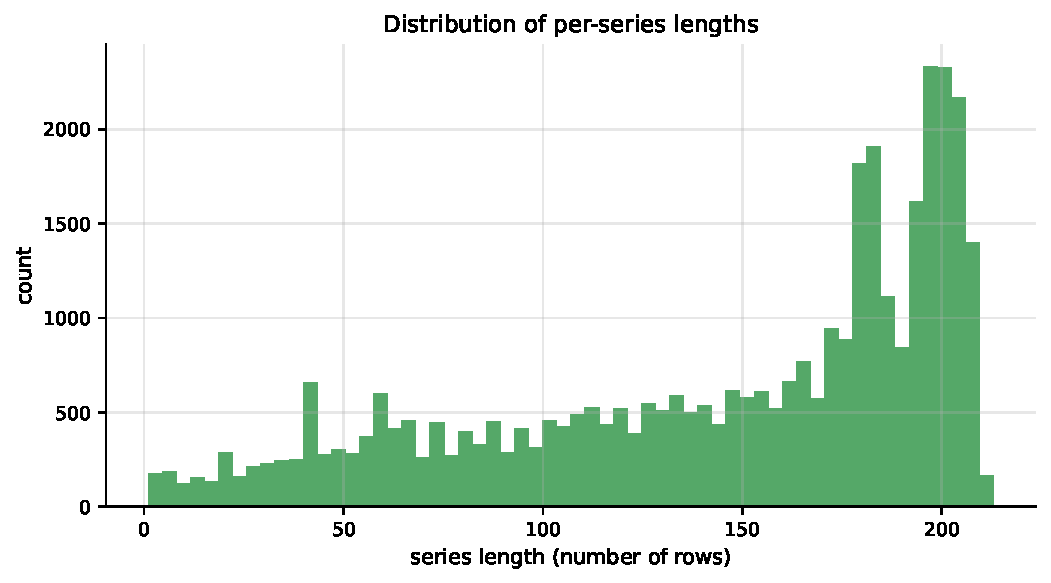
\includegraphics[width=0.85\linewidth]{00_series_length_distribution}
\caption{Distribution of per-series lengths. Most series are short, and the tail of long series carries the structural signal that classical fits can exploit.}
\label{fig:series_length}
\end{figure}

\paragraph{Reading.} Per-series classical fitting is feasible only on the eligible subset (cross the cutoff with at least 120 training rows). Global pooled models are not length-constrained --- one reason the comparison between local classical and global ML approaches is not perfectly apples-to-apples.

\subsection{Representative-series selection}
\label{sec:eda:repseries}

For every per-series figure in this project we plot the same four series. They are selected with explicit reasons rather than at random, in order to span four distinct stress regimes: long history, large weight, high variability, and near-flat behaviour. \Cref{tab:representative} lists the four chosen series. They match the selection used in the midway report, preserving visual continuity.

\begin{table}[h]
\centering
\caption{Four representative series chosen for per-series studies. Each series probes a different regime of the panel.}
\label{tab:representative}
\begin{tabular}{l l l c}
\toprule
Reason & Series key (code/sub\_code) & Horizon & Length \\
\midrule
Longest history       & X9BZ68VQ / OYJGNSQK / DPPUO5X2 & 1  & 212 \\
Highest total weight  & SJZP0OVU / OYJGNSQK / NQ58FVQM & 25 & 156 \\
Most volatile         & W4S29LF4 / KL66VIS3 / PHHHVYZI & 25 & 162 \\
Most stable           & SJZP0OVU / OYJGNSQK / NQ58FVQM & 1  & 170 \\
\bottomrule
\end{tabular}
\end{table}

\Cref{fig:rep_series_raw} shows the raw $y_{\text{target}}$ trajectory of each chosen series with the train/validation cutoff marked. The four panels look profoundly different: the most-volatile series swings between $-500$ and $+500$, while the most-stable series occupies a numerical range narrower than $0.001$.

\begin{figure}[h]
\centering
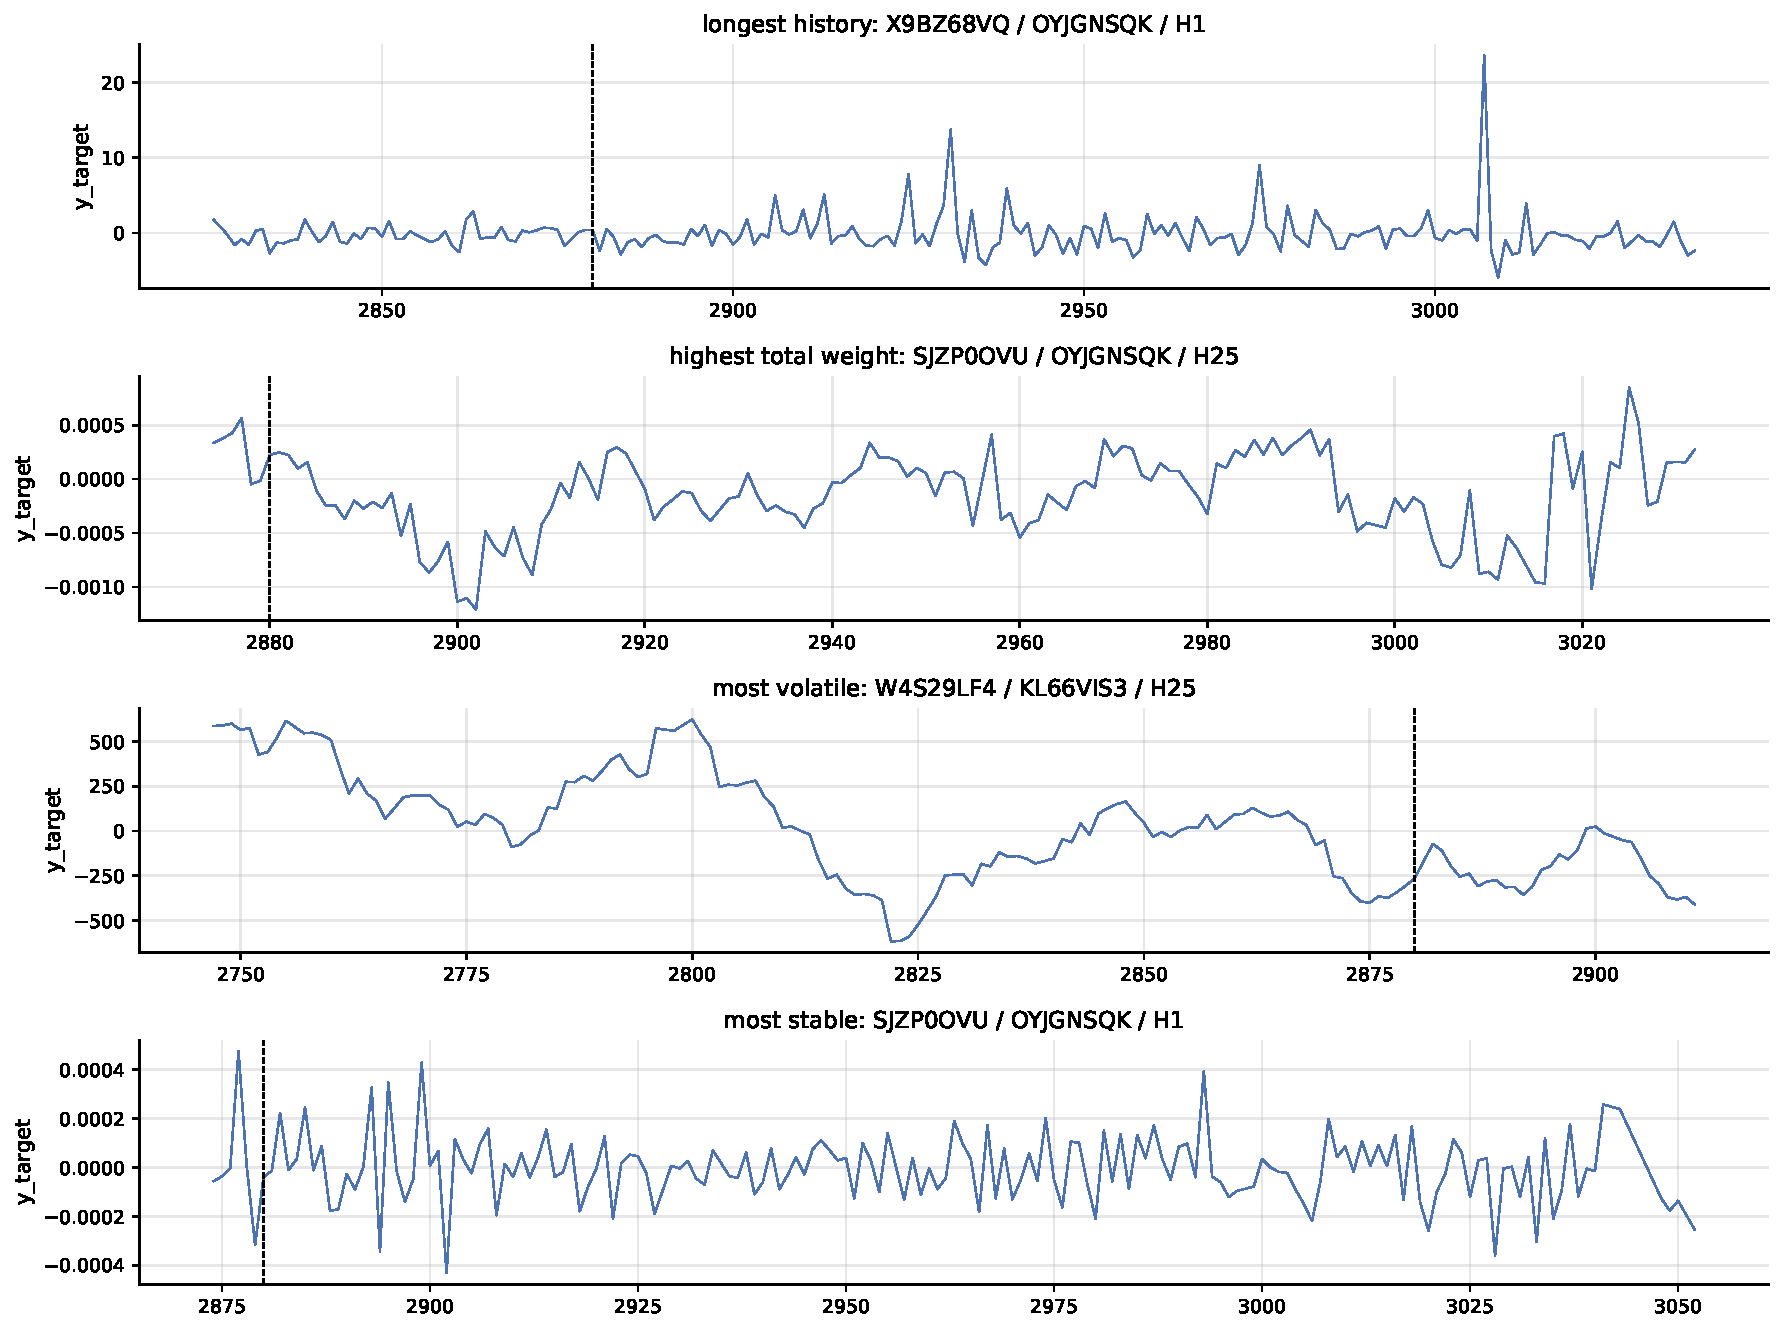
\includegraphics[width=0.95\linewidth]{00_representative_series_raw}
\caption{Raw $y_{\text{target}}$ for the four chosen representative series. The dashed vertical line marks $\mathtt{ts\_index} = 2880$, the train/validation cutoff. The four panels span the four stress regimes that any model has to handle.}
\label{fig:rep_series_raw}
\end{figure}

\paragraph{Reading.} A one-size-fits-all model will struggle: the most-stable series is essentially numerical noise, while the most-volatile series has obvious cyclical structure. Forecast performance across these four panels is one of the cleanest diagnostics for whether a model family generalises or only fits one regime.

\subsection{Stationarity diagnostics}
\label{sec:eda:stationarity}

Classical ARIMA-family forecasting assumes stationarity, or stationarity-after-differencing. We therefore run the Augmented Dickey--Fuller test on a stratified sample of 200 eligible series. The ADF test takes the null hypothesis that the series has a unit root (non-stationary); we reject at the 5\% level when the $p$-value is below $0.05$. \Cref{fig:adf} summarises the results.

\begin{figure}[h]
\centering
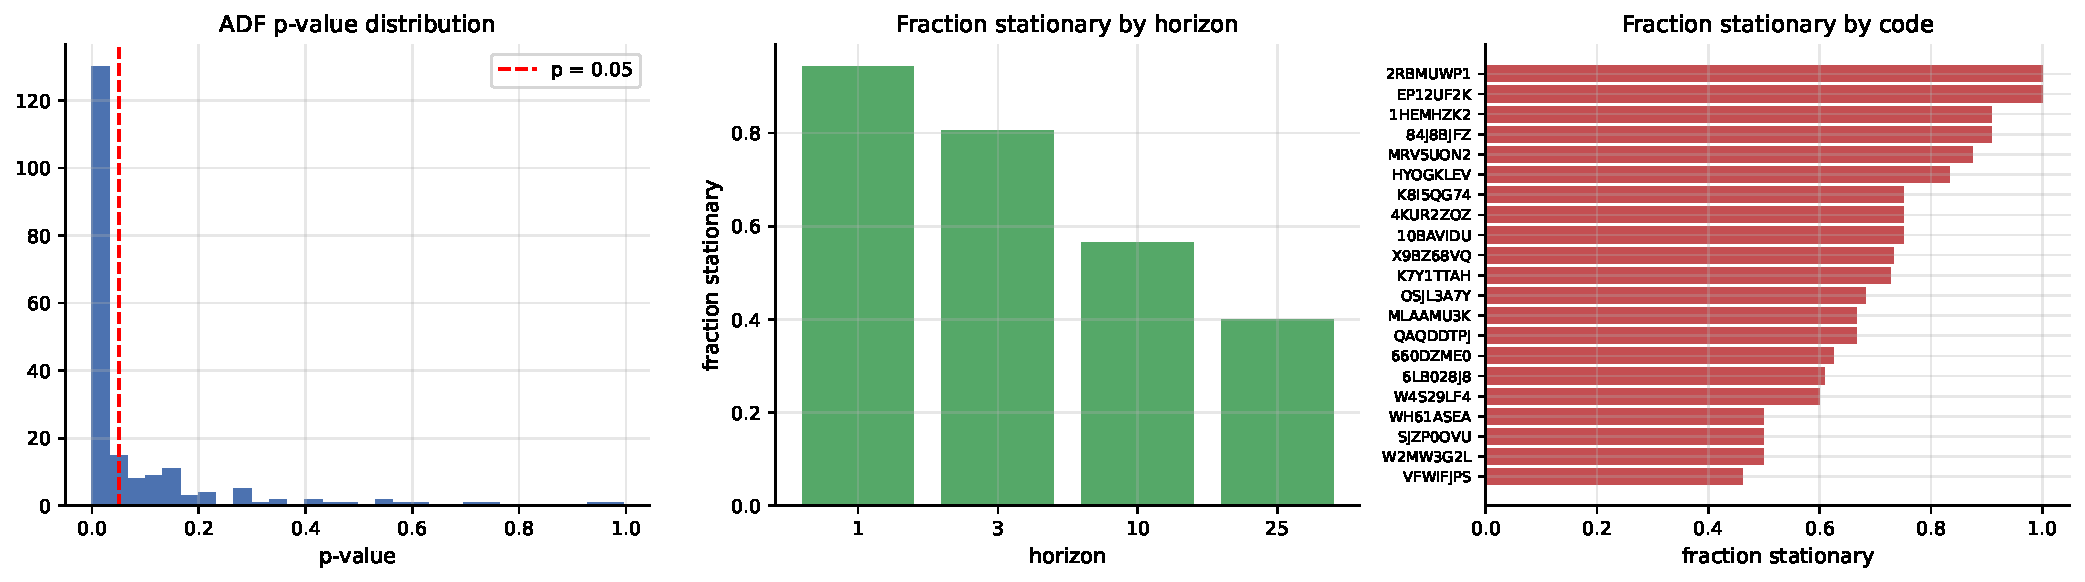
\includegraphics[width=0.95\linewidth]{00_adf_results}
\caption{ADF results on 200 sampled eligible series. Left: $p$-value distribution with the $0.05$ threshold marked. Centre: fraction stationary by horizon. Right: fraction stationary by code.}
\label{fig:adf}
\end{figure}

Approximately 70.5\% of sampled series reject the unit-root null at the 5\% level. The picture is more nuanced when broken down by horizon: H1 series are more often stationary than longer-horizon cumulative series, which is consistent with the multi-horizon coupling we will document in \cref{sec:cumulation}.

ADF and KPSS have opposite null hypotheses, so running both gives a more honest joint verdict: ADF takes non-stationarity as the null, while KPSS takes stationarity as the null. We classify a series as \emph{stationary} when ADF rejects and KPSS does not, as \emph{unit root} when ADF fails to reject and KPSS rejects, and as \emph{inconclusive} otherwise. \Cref{fig:adf_kpss} reports the joint distribution.

\begin{figure}[h]
\centering
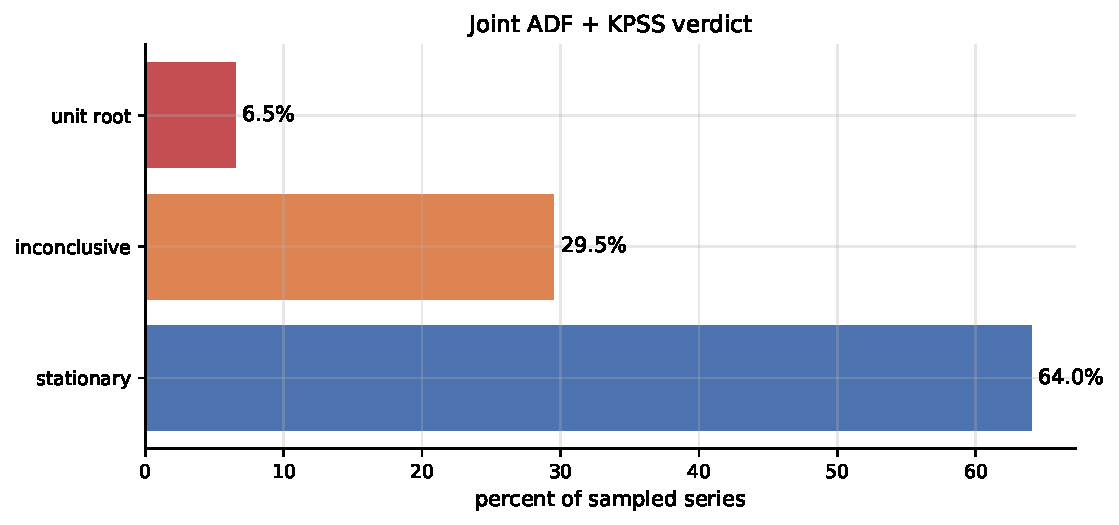
\includegraphics[width=0.7\linewidth]{00_adf_kpss_joint}
\caption{Joint ADF $+$ KPSS verdict on 200 sampled series. Stationary 64.0\%, inconclusive 29.5\%, unit root 6.5\%.}
\label{fig:adf_kpss}
\end{figure}

The stationary share dominates, but the inconclusive bucket is large enough that one-size-fits-all claims about raw levels would be unsafe. We need a repair step (differencing) for the unit-root and inconclusive cases.

\Cref{fig:differencing} re-runs the ADF test on the first-differenced series. The stationary share rises from 70.5\% on raw levels to 98.5\% after differencing.

\begin{figure}[h]
\centering
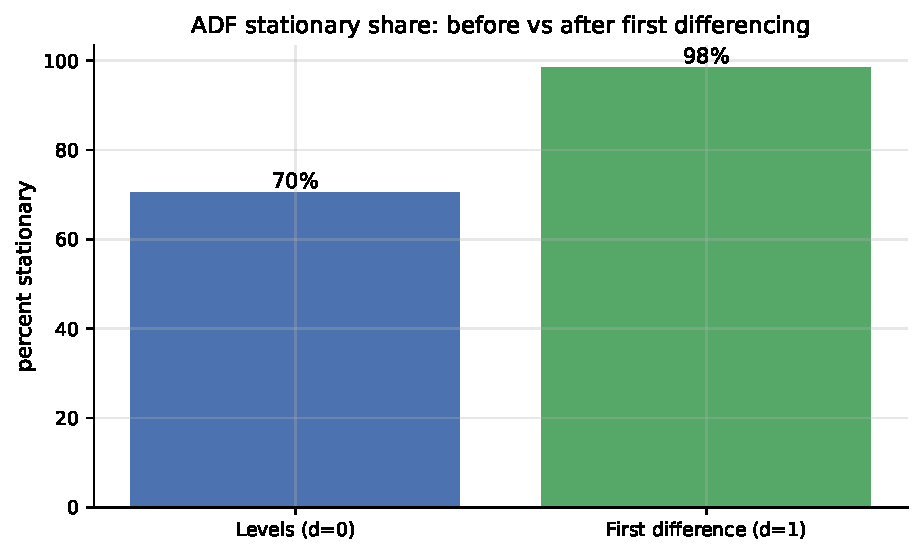
\includegraphics[width=0.7\linewidth]{00_first_differencing_share}
\caption{ADF stationary share at the 5\% level: levels (left, $d=0$) versus first differences (right, $d=1$). Differencing pushes the share to nearly 100\%.}
\label{fig:differencing}
\end{figure}

\paragraph{Reading.} The diagnostic chain motivates ARIMA with $d=1$ as the default for the classical study and justifies engineered differenced features for global ML models. The 98.5\% post-difference stationarity also bears on the cumulation finding in \cref{sec:cumulation}: differencing a higher-horizon target partially inverts the rolling-sum construction back into the H1 process.

\subsection{Visual stationarity --- rolling statistics}
\label{sec:eda:rolling}

Statistical tests can disagree on short or noisy series, so a rolling-window view is a useful visual check. \Cref{fig:rolling_raw} shows a 24-step rolling mean and rolling standard deviation on the raw four representative series. The most-volatile series shows clear drift in level and bulging variance; the longest-history series drifts upward; the high-weight and most-stable series occupy near-flat ranges where the rolling mean barely moves.

\begin{figure}[h]
\centering
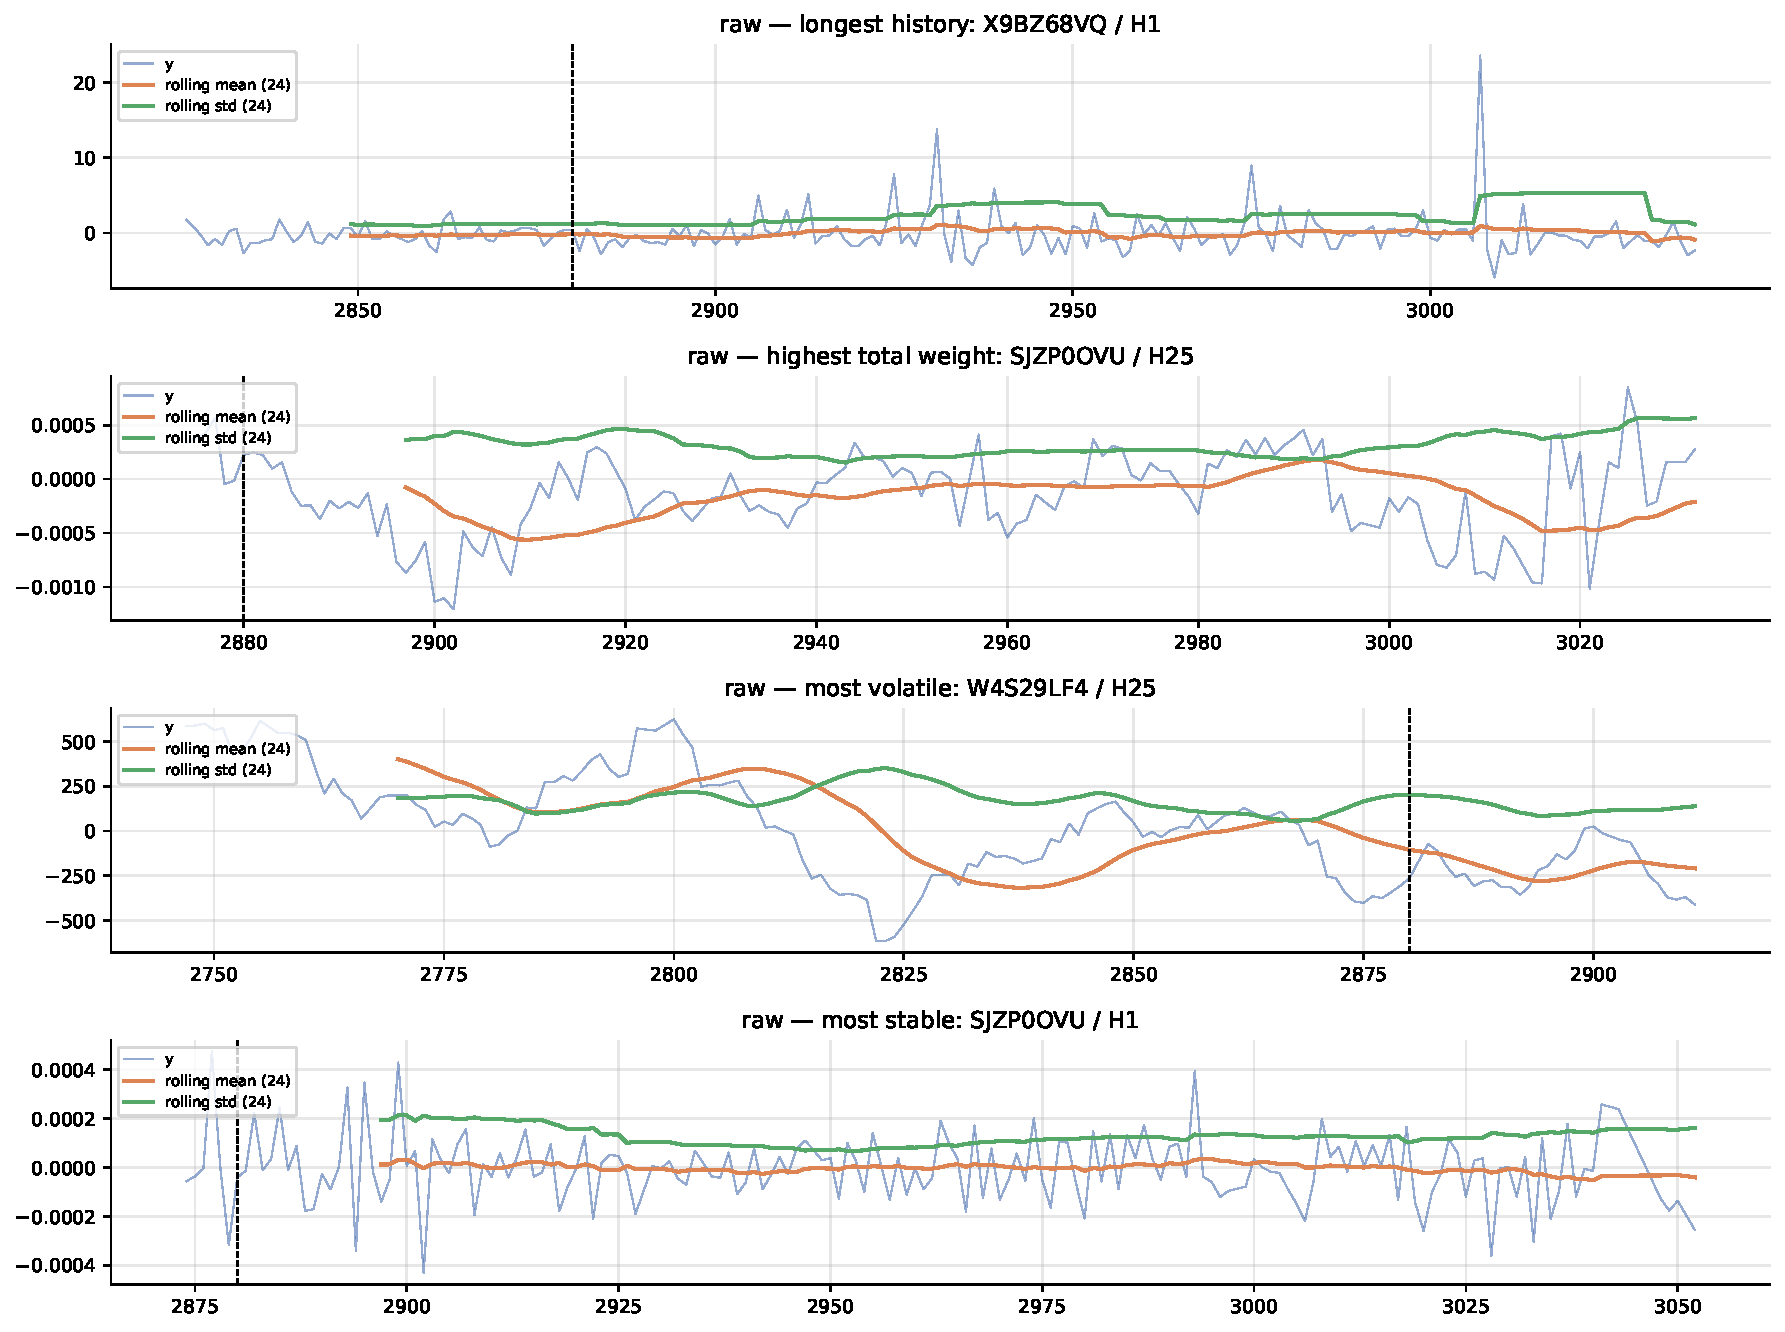
\includegraphics[width=0.95\linewidth]{00_rolling_raw}
\caption{Rolling mean and rolling standard deviation (window = 24) on the raw four representative series. The most-volatile series shows clear drift in level and bulging variance.}
\label{fig:rolling_raw}
\end{figure}

\Cref{fig:rolling_diff} repeats the same diagnostic on the first-differenced versions of the same series. The rolling means now hug zero and the rolling standard deviations flatten across the cutoff, visually confirming the statistical jump from the previous subsection.

\begin{figure}[h]
\centering
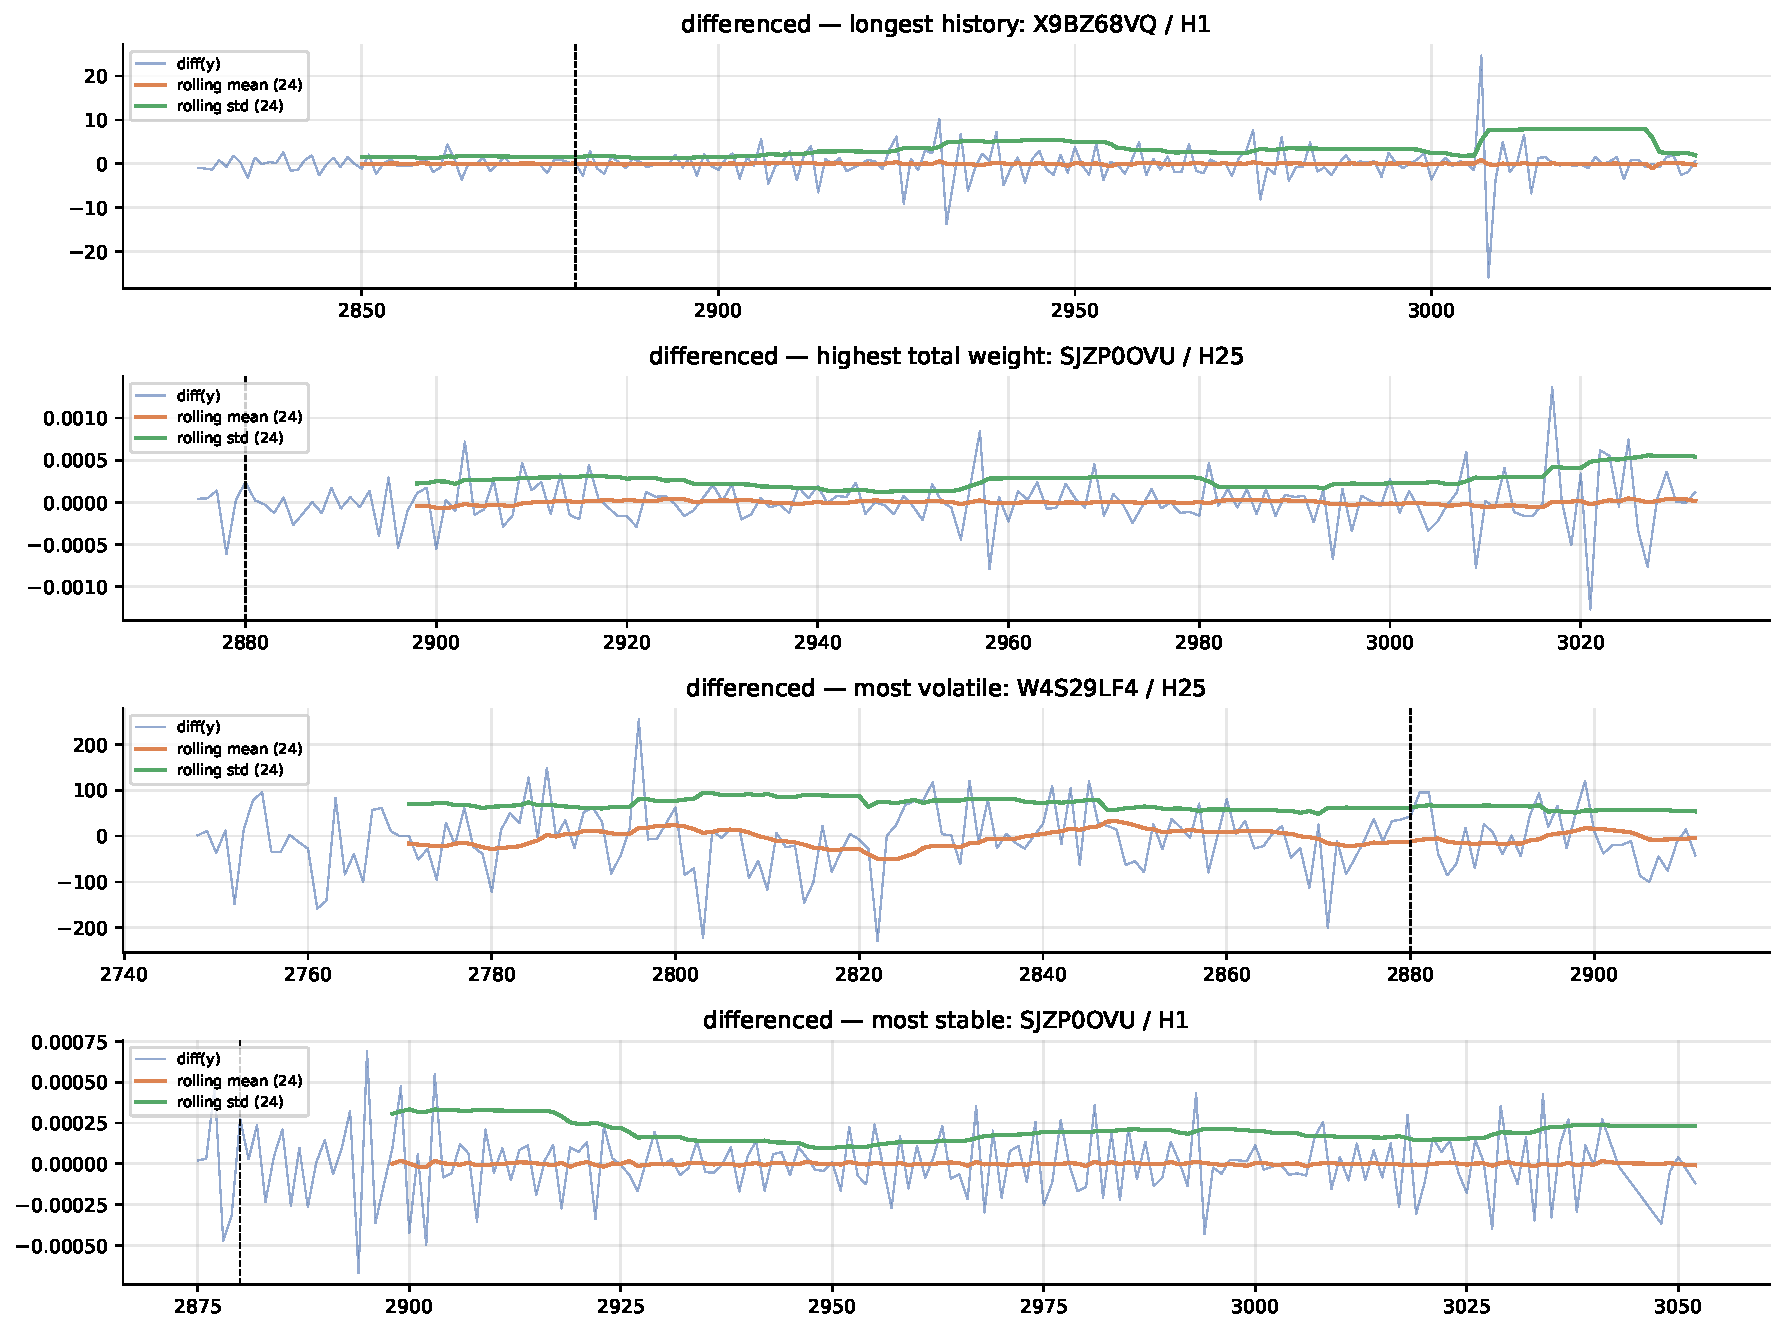
\includegraphics[width=0.95\linewidth]{00_rolling_differenced}
\caption{Rolling mean and rolling standard deviation (window = 24) on the first-differenced four representative series. The mean oscillates close to zero and the variance is stable, consistent with stationarity.}
\label{fig:rolling_diff}
\end{figure}

\paragraph{Reading.} Differenced series behave like the white-noise regime we want before fitting a differenced classical model.

\subsection{Lag structure --- ACF and PACF}
\label{sec:eda:acf}

The autocorrelation function (ACF) shows correlation between the series and lagged copies of itself; the partial autocorrelation function (PACF) isolates each lag's direct contribution after controlling for shorter lags. A sharp PACF cutoff suggests an autoregressive order; a sharp ACF cutoff suggests a moving-average order. Rather than relying on a single anchor series, we aggregate the absolute ACF and PACF across all 200 sampled eligible series (\cref{fig:acf_panel}). The panel-level view exposes which lags are reliably informative across the panel rather than artefacts of one trajectory.

\begin{figure}[h]
\centering
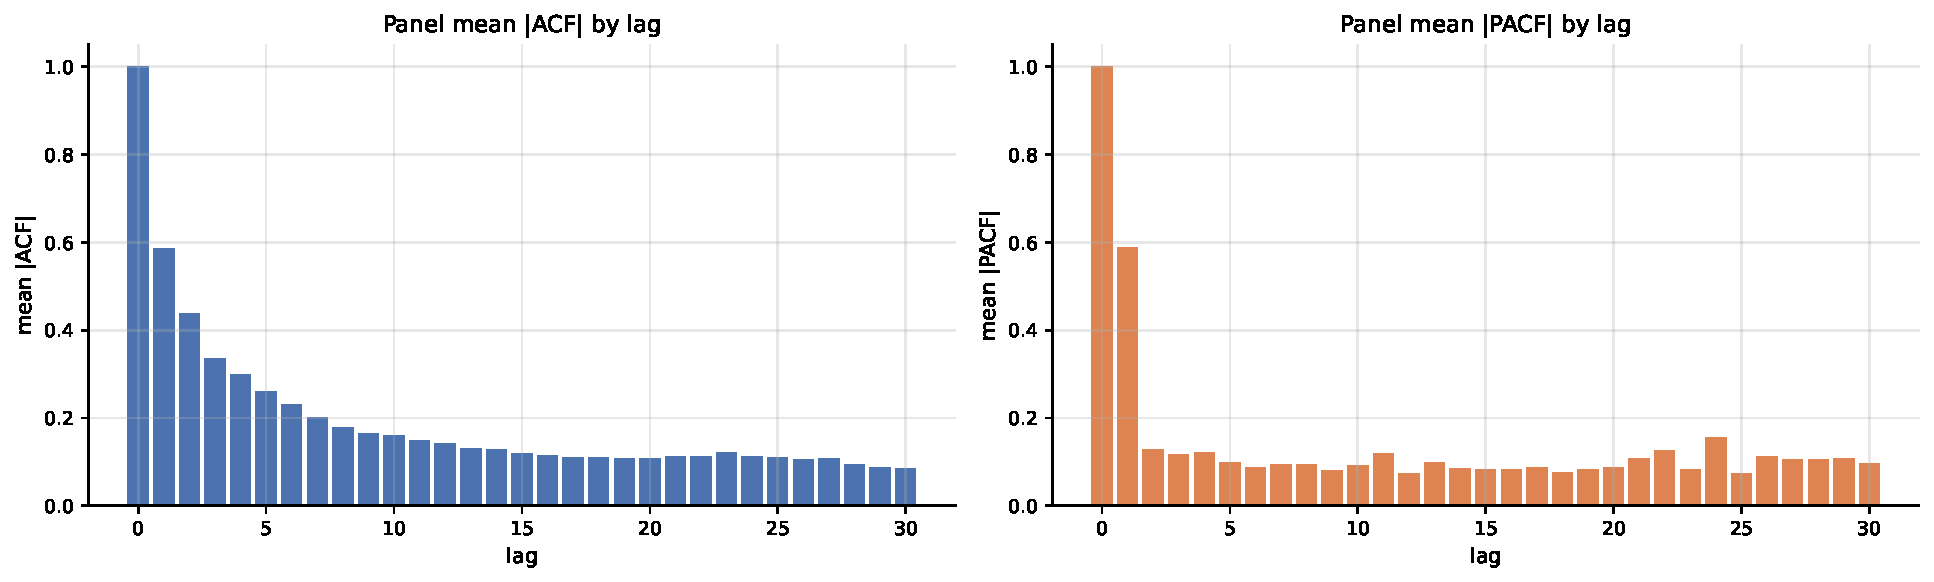
\includegraphics[width=0.95\linewidth]{00_acf_pacf_panel}
\caption{Panel-level mean $|\text{ACF}|$ (left) and mean $|\text{PACF}|$ (right) across 200 sampled eligible series. Persistent low-order lags dominate; higher lags decay quickly. There are no clean seasonal bumps.}
\label{fig:acf_panel}
\end{figure}

\paragraph{Reading.} Short-memory dynamics dominate (lags 1--3 carry most of the structure with rapid decay thereafter), and there are no clean seasonal bumps. The lag feature set for the global ML models therefore prioritises lags 1, 2, 3, 5, 10 and skips seasonal indicators.

\subsection{STL decomposition}
\label{sec:eda:stl}

Seasonal-Trend decomposition using LOESS (STL) splits a series into trend, seasonal, and residual components. We apply STL to the longest-history anchor with a period of 24 and observe the relative amplitudes of the three components. \Cref{fig:stl} shows the result.

\begin{figure}[h]
\centering
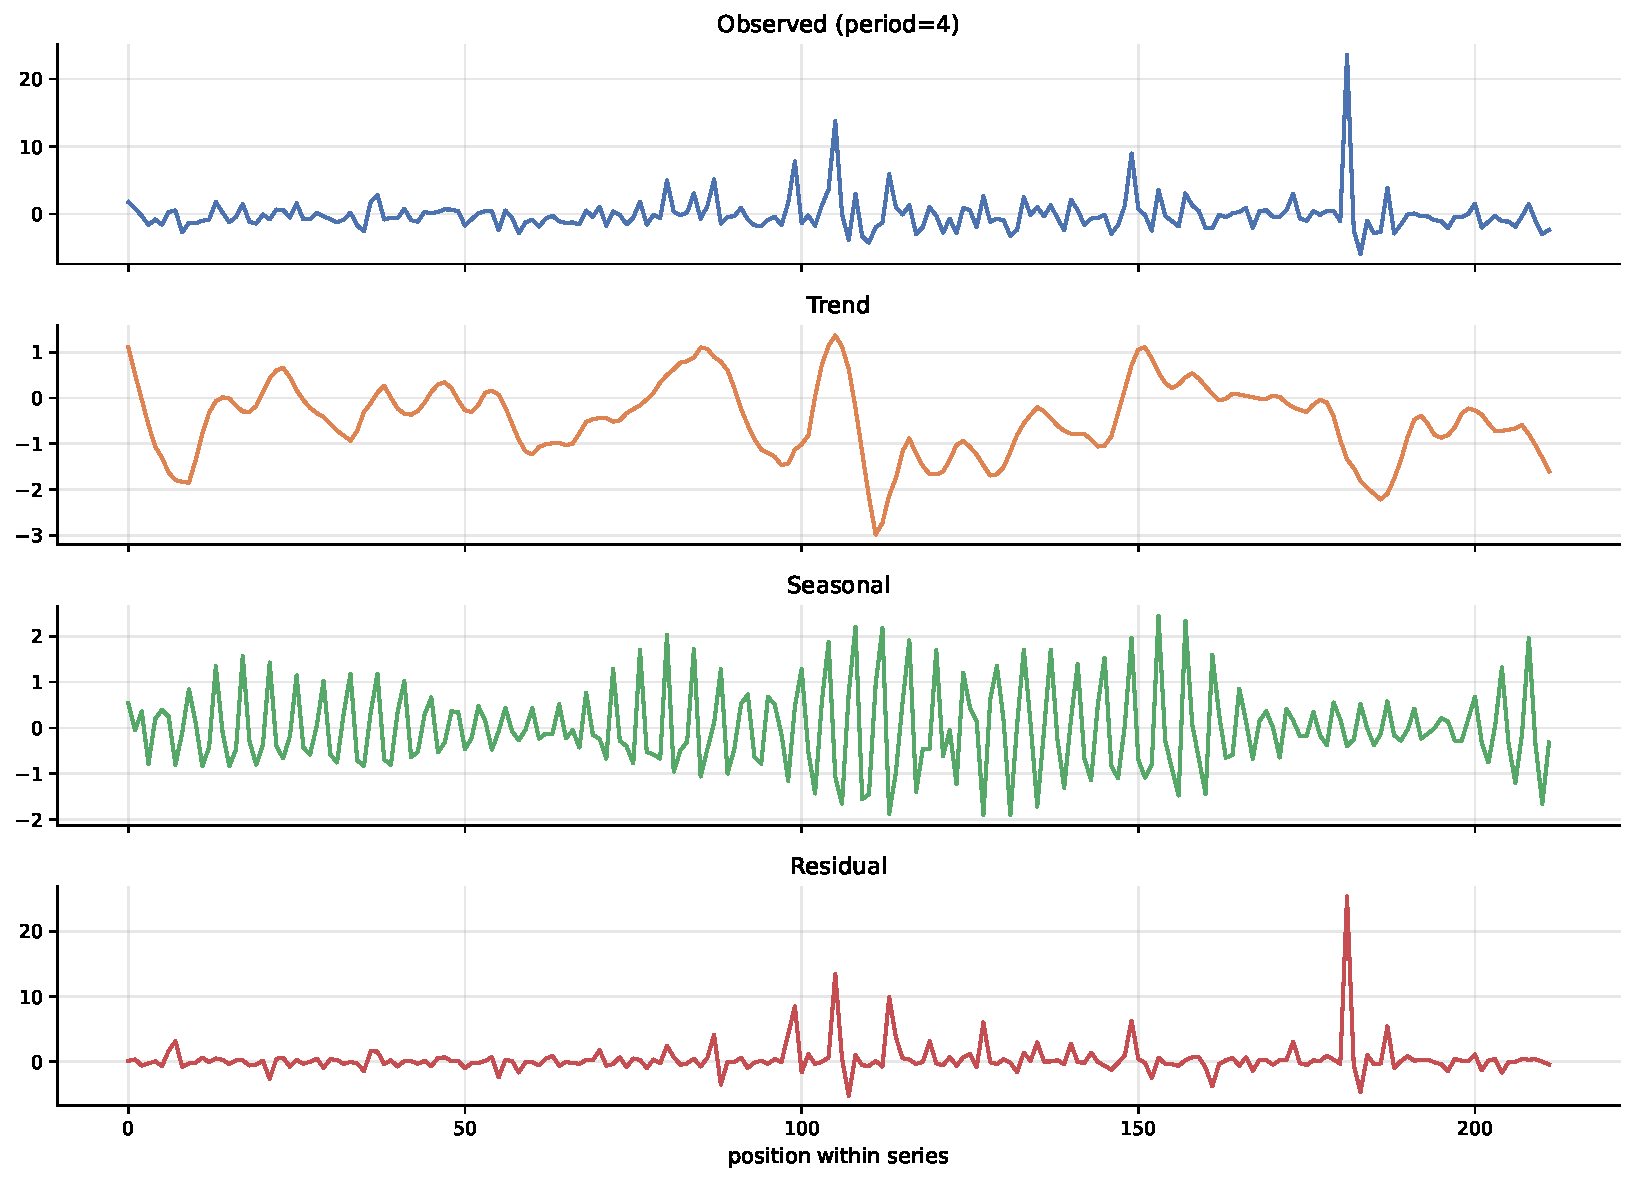
\includegraphics[width=0.85\linewidth]{00_stl_anchor}
\caption{STL decomposition of the longest-history anchor with period 24. The trend component captures slow drift; the seasonal amplitude is small relative to residual standard deviation.}
\label{fig:stl}
\end{figure}

\paragraph{Reading.} The trend captures slow drift, but the seasonal amplitude is small relative to the residual. Combined with the absence of seasonal bumps in the panel ACF, this confirms periodic structure is not the dominant signal --- modelling effort goes into short-memory dynamics, not seasonal indicators.

\subsection{Feature audit}
\label{sec:eda:feature_audit}

The 86 \texttt{feature\_*} columns are anonymised and we cannot interpret them by name. We can, however, audit them statistically. On a 200{,}000-row stratified sample we compute Pearson correlation between each feature and $y_{\text{target}}$, then rank features by absolute correlation. \Cref{fig:feature_corr} shows the top twenty.

\begin{figure}[h]
\centering
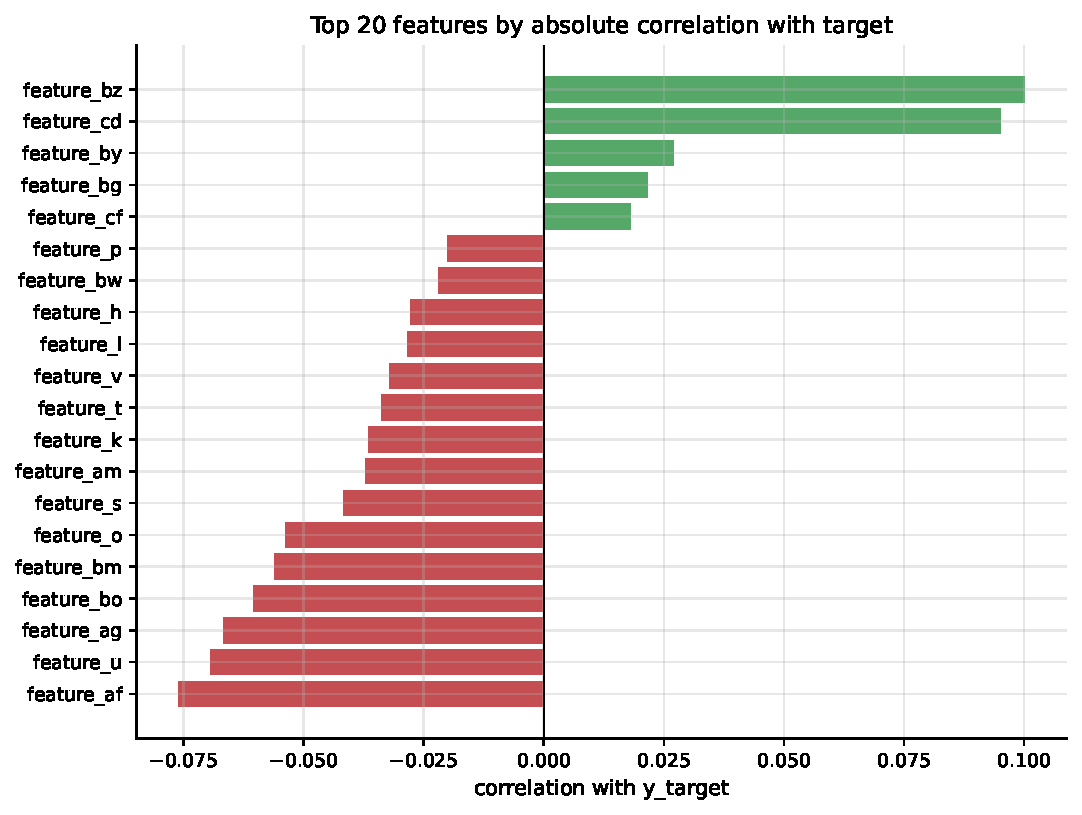
\includegraphics[width=0.85\linewidth]{00_feature_corr_top20}
\caption{Top twenty features by absolute correlation with $y_{\text{target}}$, computed on a 200{,}000-row stratified sample. Green bars are positive correlations, red bars are negative.}
\label{fig:feature_corr}
\end{figure}

\paragraph{Reading.} The single largest absolute correlation is below 0.10. No single feature predicts the target well on its own. A separate correlation check among the top twenty features further reveals strong feature--feature blocks, indicating real redundancy in the engineered set. Together these say: the signal is weak, spread across many correlated features, and best exploited by gradient-boosted trees combined with caution when reading importance plots.

\subsection{Cross-series relationships}
\label{sec:eda:cross_series}

Within the same \texttt{code}, different sub-codes might share signal. If they do, global pooled models can borrow strength across related sub-codes; per-series local models cannot. We compute lagged cross-correlations between random pairs of sub-codes within the same \texttt{(code, horizon)} group. \Cref{fig:cross_series} shows six representative pairs.

\begin{figure}[h]
\centering

\includegraphics[width=0.95\linewidth]{00_cross_series}
\caption{Lagged cross-correlation between random sub-code pairs sharing the same code and horizon. A peak away from lag 0 means one sub-code leads or lags the other.}
\label{fig:cross_series}
\end{figure}

\paragraph{Reading.} Clear lead/lag peaks within a code mean global models can learn a shared cross-sub-code component that per-series fits cannot. This is one of the strongest a-priori arguments for the global ML approach.

\subsection{Multi-horizon coupling}
\label{sec:multihorizon}

The midway report treated $(\mathtt{code},\mathtt{sub\_code},\mathtt{sub\_category},\mathtt{horizon})$ as the natural series identifier and fit each horizon independently. The exploratory analysis in this project shows that the four horizons of the same triple are not independent. For approximately 1.21 million distinct $(\mathtt{code},\mathtt{sub\_code},\mathtt{sub\_category},\mathtt{ts\_index})$ tuples, all four horizons are simultaneously present.

A second consequence of multi-horizon coupling is per-horizon target scaling. \Cref{fig:horizon_scale} shows the target standard deviation and maximum row weight by horizon.

\begin{figure}[h]
\centering
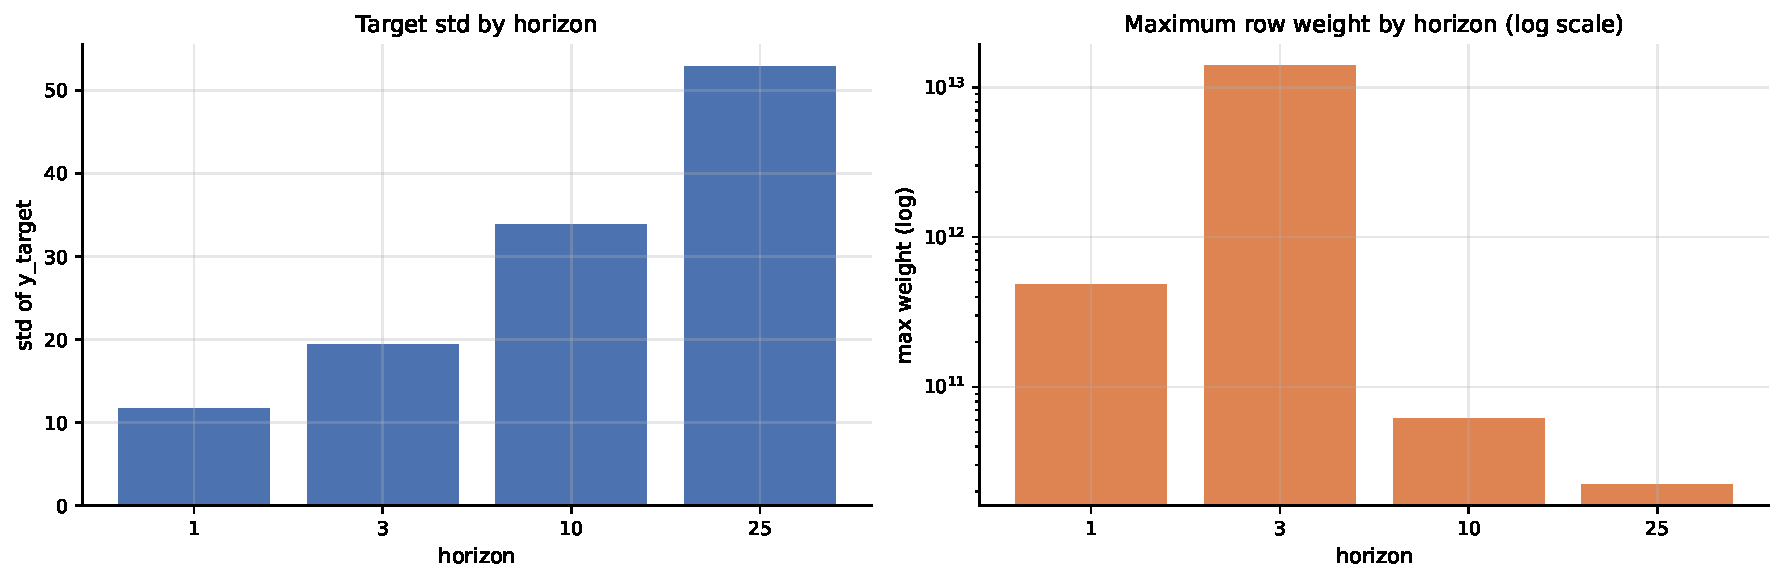
\includegraphics[width=0.95\linewidth]{00_horizon_scale_and_weight}
\caption{Per-horizon target standard deviation (left) and maximum row weight on a logarithmic scale (right). Target scale grows by a factor of approximately 4.5 from H1 to H25. Maximum weight is highest at H3.}
\label{fig:horizon_scale}
\end{figure}

The target standard deviation rises from approximately 11.7 at H1 to 52.8 at H25, a factor of $4.5$.

\paragraph{Reading.} This finding has direct modelling consequences. A single model trained on horizons pooled into one DataFrame, without horizon-aware standardisation, will be dominated by H25 magnitudes and predict at H25 scale. Predictions at H25 scale evaluated against H1 targets will overshoot by a factor of roughly 4.5, producing catastrophically large weighted RMSE on H1 rows. This is exactly the failure mode observed in earlier ML artefacts attached to the project --- the original XGBoost run reported a weighted RMSE more than two hundred times the naive baseline, consistent with a per-horizon-scale leak. The remedy is straightforward: train one model per horizon, or normalise the target by horizon before training.

\subsection{Cumulation hypothesis}
\label{sec:cumulation}

Given the multi-horizon coupling above, the natural hypothesis about how the four horizons relate to each other is that the target at horizon $k$ is a cumulative aggregate of the H1 target over the next $k$ steps:
\begin{equation}
\label{eq:cumulation}
  y^{H_k}_{t} \;\approx\; \sum_{i=0}^{k-1} y^{H_1}_{t+i}.
\end{equation}
We test \cref{eq:cumulation} on a stratified sample of 500 triples that have all four horizons and at least 60 H1 rows. For each triple we pivot the data so that horizons sit on columns, compute the rolling sum of the H1 series over the appropriate window, and report the Pearson correlation between $y^{H_k}_t$ and that rolling sum. \Cref{fig:cumulation} shows the distribution of correlations and the median ratio.

\begin{figure}[h]
\centering
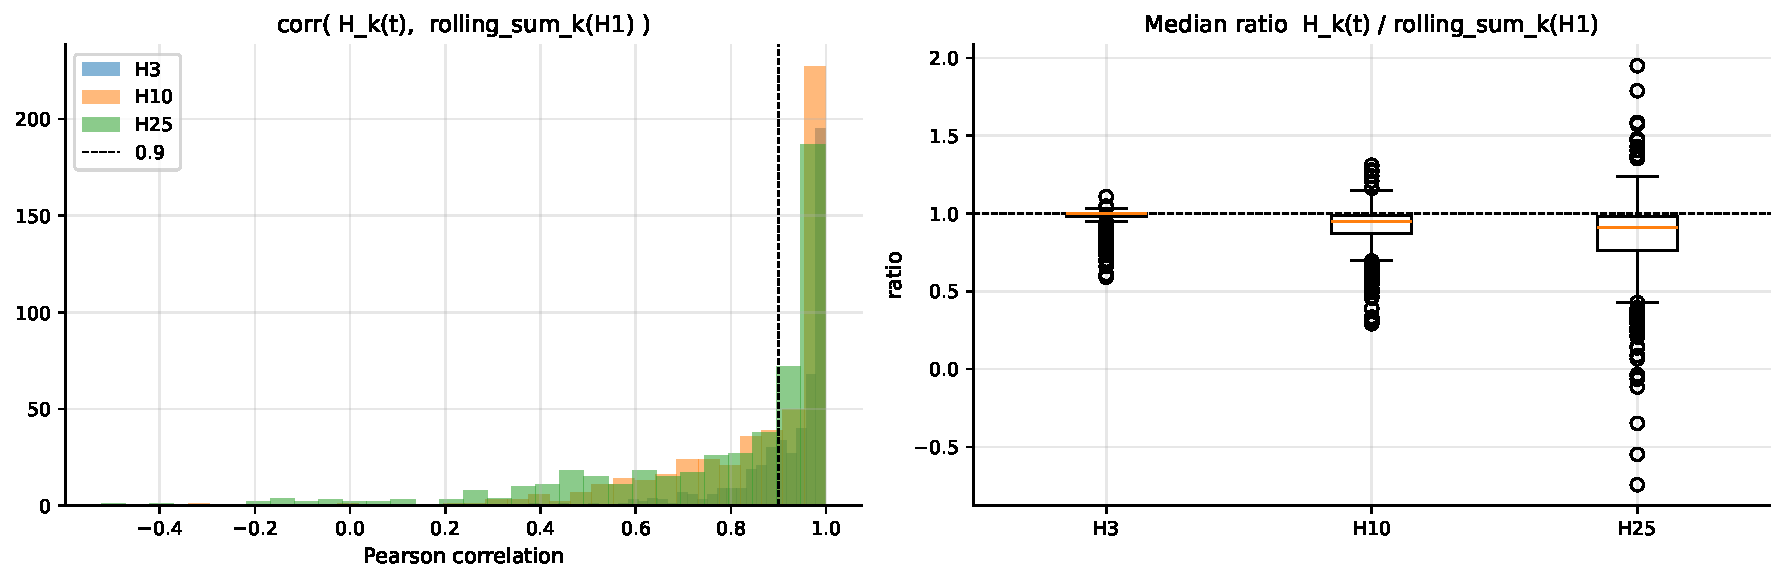
\includegraphics[width=0.95\linewidth]{00_cumulation_hypothesis}
\caption{Test of the cumulation hypothesis on 500 stratified triples. Left: distribution of Pearson correlations between $y^{H_k}_t$ and the rolling sum of $y^{H_1}$ over $k$ steps, for $k \in \{3, 10, 25\}$. Right: distribution of the per-triple median ratio $y^{H_k}_t / \sum y^{H_1}$. Higher and tighter is better.}
\label{fig:cumulation}
\end{figure}

\Cref{tab:cumulation} reports the summary statistics. At $k=3$ the median Pearson correlation is 0.96 and the median ratio is 1.00, indicating essentially exact aggregation. The relation is slightly noisier at $k=10$ and $k=25$, with median ratios of 0.95 and 0.91, but still clearly dominant.

\begin{table}[h]
\centering
\caption{Cumulation hypothesis test summary on 500 triples.}
\label{tab:cumulation}
\begin{tabular}{c r r r r}
\toprule
$k$ & $n$ triples & mean corr & median corr & median ratio \\
\midrule
3   & 500 & 0.92 & 0.96 & 1.00 \\
10  & 500 & 0.86 & 0.94 & 0.95 \\
25  & 500 & 0.78 & 0.91 & 0.91 \\
\bottomrule
\end{tabular}
\end{table}

\paragraph{Reading.} Two consequences for the modelling work that follows. First, fit-H1-and-aggregate becomes a viable, possibly superior strategy to fitting per-horizon models independently: a single H1 model gives H3, H10, and H25 forecasts for free, and the aggregation is mathematically forced by the data construction. We test this in a dedicated H1-aggregation experiment in a later notebook. Second, differencing operations on $y^{H_{25}}$ partially recover the $y^{H_1}$ process, which explains why ARIMA with $d=1$ wins the most-volatile H25 series in the midway classical study: differencing inverts the cumulation. The midway interpretation that ARIMA was capturing a difficult pattern is partly correct; it was also undoing the cumulative construction.

\subsection{Per-horizon weight dominance}
\label{sec:weight_per_horizon}

The weight distribution analysis in \cref{sec:weight_dist} was panel-wide. Because $\mathtt{weight}$ and $\mathtt{horizon}$ are correlated, the rows that drive the weighted skill score may not be evenly distributed across horizons. \Cref{fig:weight_horizon} reports the share of total panel weight per horizon and the share of weight within the top 1\% of all weight mass.

\begin{figure}[h]
\centering
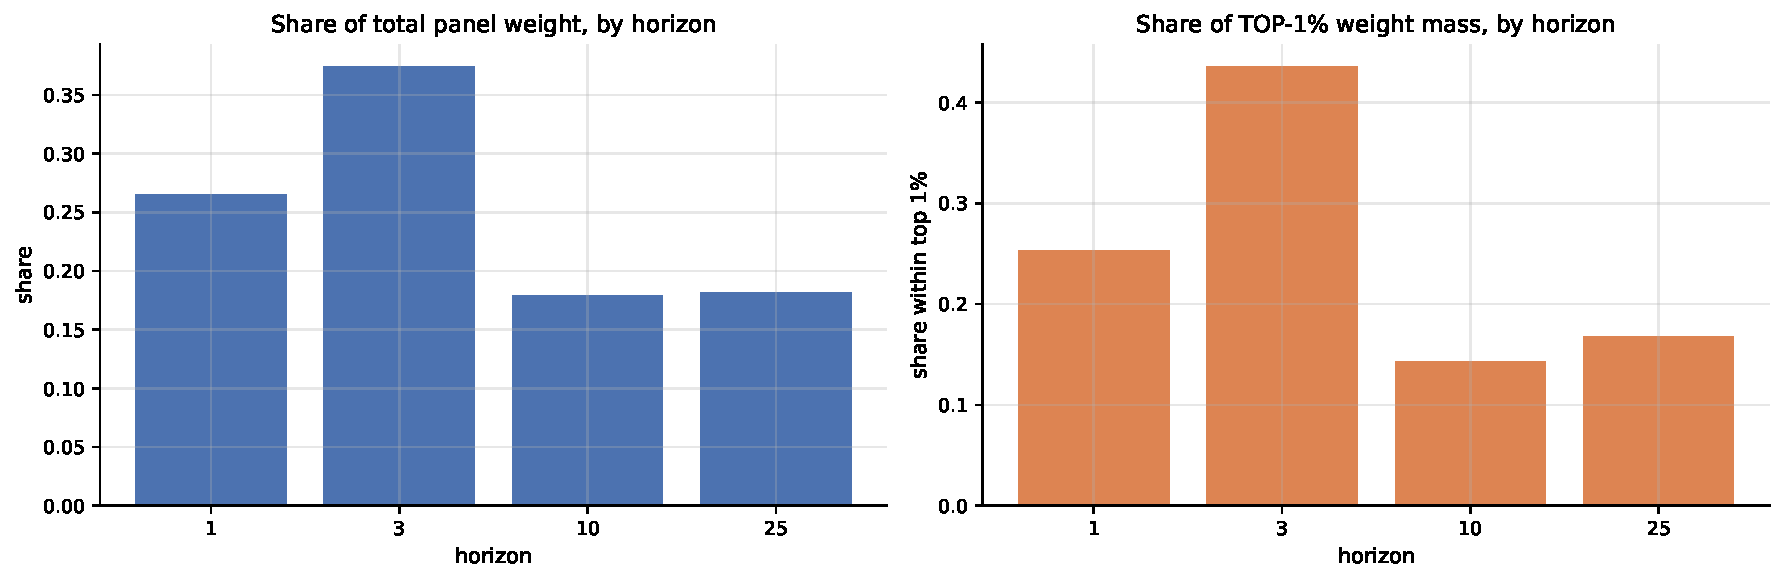
\includegraphics[width=0.95\linewidth]{00_weight_by_horizon}
\caption{Per-horizon weight breakdown. Left: each horizon's share of total panel weight. Right: share of the top 1\% of weight mass by horizon. H3 dominates both views.}
\label{fig:weight_horizon}
\end{figure}

The headline numbers are striking. The maximum panel weight ($1.39 \times 10^{13}$) is at H3, not H1. H3 alone holds 37.4\% of total panel weight and 43.6\% of the top-1\% weight mass; H1 holds 25.4\%, H10 holds 14.3\%, and H25 holds 16.8\%.

\paragraph{Reading.} A model that predicts H3 well on the small set of high-weight rows will tend to win the leaderboard regardless of how it performs on the other horizons. This was missed in the midway report. The practical consequence is that we report H3 weighted skill as a separate headline number alongside the panel-wide score, and we track H3 performance carefully when comparing models.

\subsection{EDA-driven modelling implications}
\label{sec:eda:implications}

The EDA findings above constrain every modelling chapter that follows. The classical baselines (notebook 01) honour the chronological cutoff and use the four representative series. The global LightGBM models (notebook 02) train per horizon with sample weights, motivated by the per-horizon target scaling and H3 weight dominance. The H1-aggregation experiment (notebook 03) operationalises the cumulation hypothesis. The probabilistic forecasting work (notebook 04) addresses the heavy tails and weak per-feature signal directly through quantile regression and conformal calibration. The ensembles (notebook 05) fit weights on a meta slice that respects chronology. The final comparison (notebook 06) reports both panel-wide and H3-specific weighted skill scores with bootstrap intervals.

\section{Classical Baselines}
\label{sec:classical}

This section establishes what per-series classical fitting can and cannot do on this panel. The four representative series from \cref{sec:eda:repseries} are forecast under a single chronological protocol, scored under the weighted skill score, and compared against naive baselines that act as the visible floor. The headline finding is that classical local fits are \emph{feasibility-limited and signal-limited}: only one of the four series produces a statistically significant improvement over the naive floor. We treat this section primarily as a scope demonstration that motivates the global pooled approach in \cref{sec:eda:cross_series} (and the modelling chapters that follow).

\subsection{Setup and the four representative series}
\label{sec:classical:setup}

We reuse the four series chosen in \cref{sec:eda:repseries} so that the visualisations carry over from the EDA. Two implementation choices differ from the midway report.

First, we use \textbf{adaptive 80/20 chronological splits per series} rather than the canonical fixed cutoff at $\mathtt{ts\_index} = 2880$. Under the fixed cutoff, two of the four series (highest-weight and most-stable) end up with only 7 pre-cutoff training points, which is below the minimum window required for ARMA/ARIMA estimation and forces those families to be skipped entirely. Adaptive splits preserve chronology --- training rows always strictly precede validation rows --- while ensuring every series has a usable training segment. The trade-off is that classical numbers in this section are not directly comparable, slice-for-slice, with the global ML numbers in later sections; we flag this explicitly when synthesising results in \cref{sec:weight_per_horizon}.

Second, we use \textbf{AICc-based automatic order selection} for AR, MA, ARMA, and ARIMA over a small grid of $(p, q) \in \{0, 1, 2, 3\}^2$. Hand-picking a winner from a 12-cell grid inflates the multiple-comparisons risk. AICc selects one order per series per family using a small-sample-corrected information criterion, so the model reported as ``the AR result'' is the one AICc would have chosen on the training data alone.

\Cref{tab:classical_splits} summarises the per-series training and validation lengths under the adaptive split.

\begin{table}[h]
\centering
\caption{Adaptive per-series chronological splits used for the classical study.}
\label{tab:classical_splits}
\begin{tabular}{l c c c c}
\toprule
Series & Horizon & Train length & Val length & Validation range \\
\midrule
Longest history     & H1  & 169 & 43 & 2995--3037 \\
Highest total weight & H25 & 124 & 32 & 3001--3032 \\
Most volatile       & H25 & 129 & 33 & 2879--2911 \\
Most stable         & H1  & 136 & 34 & 3013--3052 \\
\bottomrule
\end{tabular}
\end{table}

\subsection{Model lineup}
\label{sec:classical:lineup}

The lineup spans naive baselines (the floor), smoothing models (robust on tiny windows), and four flavours of order-selected ARIMA-family models.

\begin{table}[h]
\centering
\caption{Classical model lineup. AR / MA / ARMA / ARIMA orders are selected per series by AICc on the grid $(p,q) \in \{0,1,2,3\}^2$ with the indicated $d$.}
\label{tab:classical_lineup}
\begin{tabular}{l l l}
\toprule
Family & Models & Role \\
\midrule
Naive baselines & Zero, Naive (lag-1), Drift     & Skill floor \\
Smoothing       & Rolling Mean ($w{=}10$), SES, Holt & Robust on small windows \\
AR              & order $(p,0,0)$, AICc-selected     & Lagged-target dependence only \\
MA              & order $(0,0,q)$, AICc-selected     & Serially correlated shocks \\
ARMA            & order $(p,0,q)$, AICc-selected     & AR + MA in levels \\
ARIMA           & order $(p,1,q)$, AICc-selected     & Differencing as the EDA-motivated repair \\
\bottomrule
\end{tabular}
\end{table}

We deliberately exclude SARIMA because the panel ACF in \cref{sec:eda:acf} shows no clean seasonal structure, so any seasonal period would be an unjustified hyperparameter. We also exclude AR/MA/ARMA/ARIMA orders larger than 3 because validation segments are 32--43 rows --- larger orders cannot be reliably estimated on this much data even when they fit the training window.

\subsection{Evaluation protocol}
\label{sec:classical:protocol}

Each model is fit on the per-series training segment and forecasts the full validation segment in one closed-form multi-step pass. This is the deployment-realistic protocol: no ground-truth feedback during forecasting. The headline number for every model is its weighted skill score on the validation segment under this protocol.

For ARIMA-family winners we additionally compute an \emph{open-loop one-step} prediction at each validation time step --- the model is given the true previous value at each step rather than its own previous prediction. Open-loop one-step is not a deployable protocol (the truth is unavailable at inference), but the gap between the two predictions is informative: it measures how much skill is lost when the model has to feed back its own predictions through the validation window. We render the one-step variant as a point cloud overlaid on the multi-step forecast in \cref{fig:classical_overlay}, but do not promote it to a headline number. For the smoothing-family winners, the open-loop one-step prediction coincides with the multi-step forecast when the smoothing parameters are estimated on training data only, so we omit it.

We deliberately do not report unweighted RMSE or MAE as headline numbers: per the discussion in \cref{sec:skill}, unweighted error metrics can disagree with the weighted skill score on which model is best, because the high-weight rows dominate the weighted score.

\subsection{Per-series leaderboard}
\label{sec:classical:leaderboard}

\Cref{tab:classical_leaderboard} reports the best model per series under weighted skill, with 95\% bootstrap confidence intervals from 500 resamples of the validation rows. The Naive (lag-1) skill is shown alongside as the floor that any reported result has to clear. Auto-selected ARIMA-family orders are shown in parentheses.

\begin{table}[h]
\centering
\caption{Per-series leaderboard under the adaptive split. ``Skill (95\% CI)'' is the weighted skill of the best model with a 500-sample bootstrap interval. ``Naive floor'' is the weighted skill of the lag-1 forecast on the same validation segment.}
\label{tab:classical_leaderboard}
\begin{tabular}{l l l c c}
\toprule
Series & Best model & Family & Skill (95\% CI) & Naive floor \\
\midrule
Longest history     & AR$(3,0,0)$        & AR        & $0.04$ \,$[0.00, 0.27]$ & $0.00$ \\
Highest total weight & SES                & Smoothing & $0.47$ \,$[0.00, 0.65]$ & $0.44$ \\
Most volatile       & Rolling Mean $(w{=}10)$ & Smoothing & $\mathbf{0.80}$ \,$[\mathbf{0.56}, \mathbf{0.91}]$ & $0.67$ \\
Most stable         & Rolling Mean $(w{=}10)$ & Smoothing & $0.17$ \,$[0.00, 0.27]$ & $0.00$ \\
\bottomrule
\end{tabular}
\end{table}

The bootstrap intervals are the substantive part of this table. Three of the four series have intervals that include zero, meaning the apparent improvement over the naive floor is within sampling noise on a validation segment of 32--43 rows. The most-volatile series is the only case where the interval excludes zero: rolling-mean skill $0.80$ with $\mathrm{CI}\,[0.56, 0.91]$ is a real positive result. For the highest-weight series the SES point estimate ($0.47$) is barely above naive ($0.44$); the wide CI down to $0.00$ confirms that the apparent edge is fragile.

A second informative signal is which family wins. Smoothing wins three of four cases, and the only AR-family winner (longest history, AR$(3,0,0)$) has the lowest skill of the four. Differenced ARIMA, which won the corresponding case in the midway report, does not appear in this leaderboard.

\subsection{Skip-status under adaptive splits}
\label{sec:classical:skip}

Under the adaptive 80/20 split, every model in the lineup successfully fits on every series. The skip-status table is therefore empty, which is itself the point of using adaptive splits: the same lineup under the canonical fixed cutoff at $\mathtt{ts\_index} = 2880$ would have skipped every ARMA, ARIMA, AR$(p \ge 2)$, and MA$(q \ge 2)$ fit on the highest-weight and most-stable series, because their pre-cutoff training segments contain only 7 rows. Reporting fit feasibility separately from fit performance is therefore unnecessary here.

\subsection{Forecast overlays}
\label{sec:classical:overlay}

\Cref{fig:classical_overlay} shows the per-series train and validation segments alongside the best model's closed-form multi-step forecast, the Naive (lag-1) floor, and (where the best model is in the AR family) the open-loop one-step variant rendered as small dots.

\begin{figure}[h]
\centering
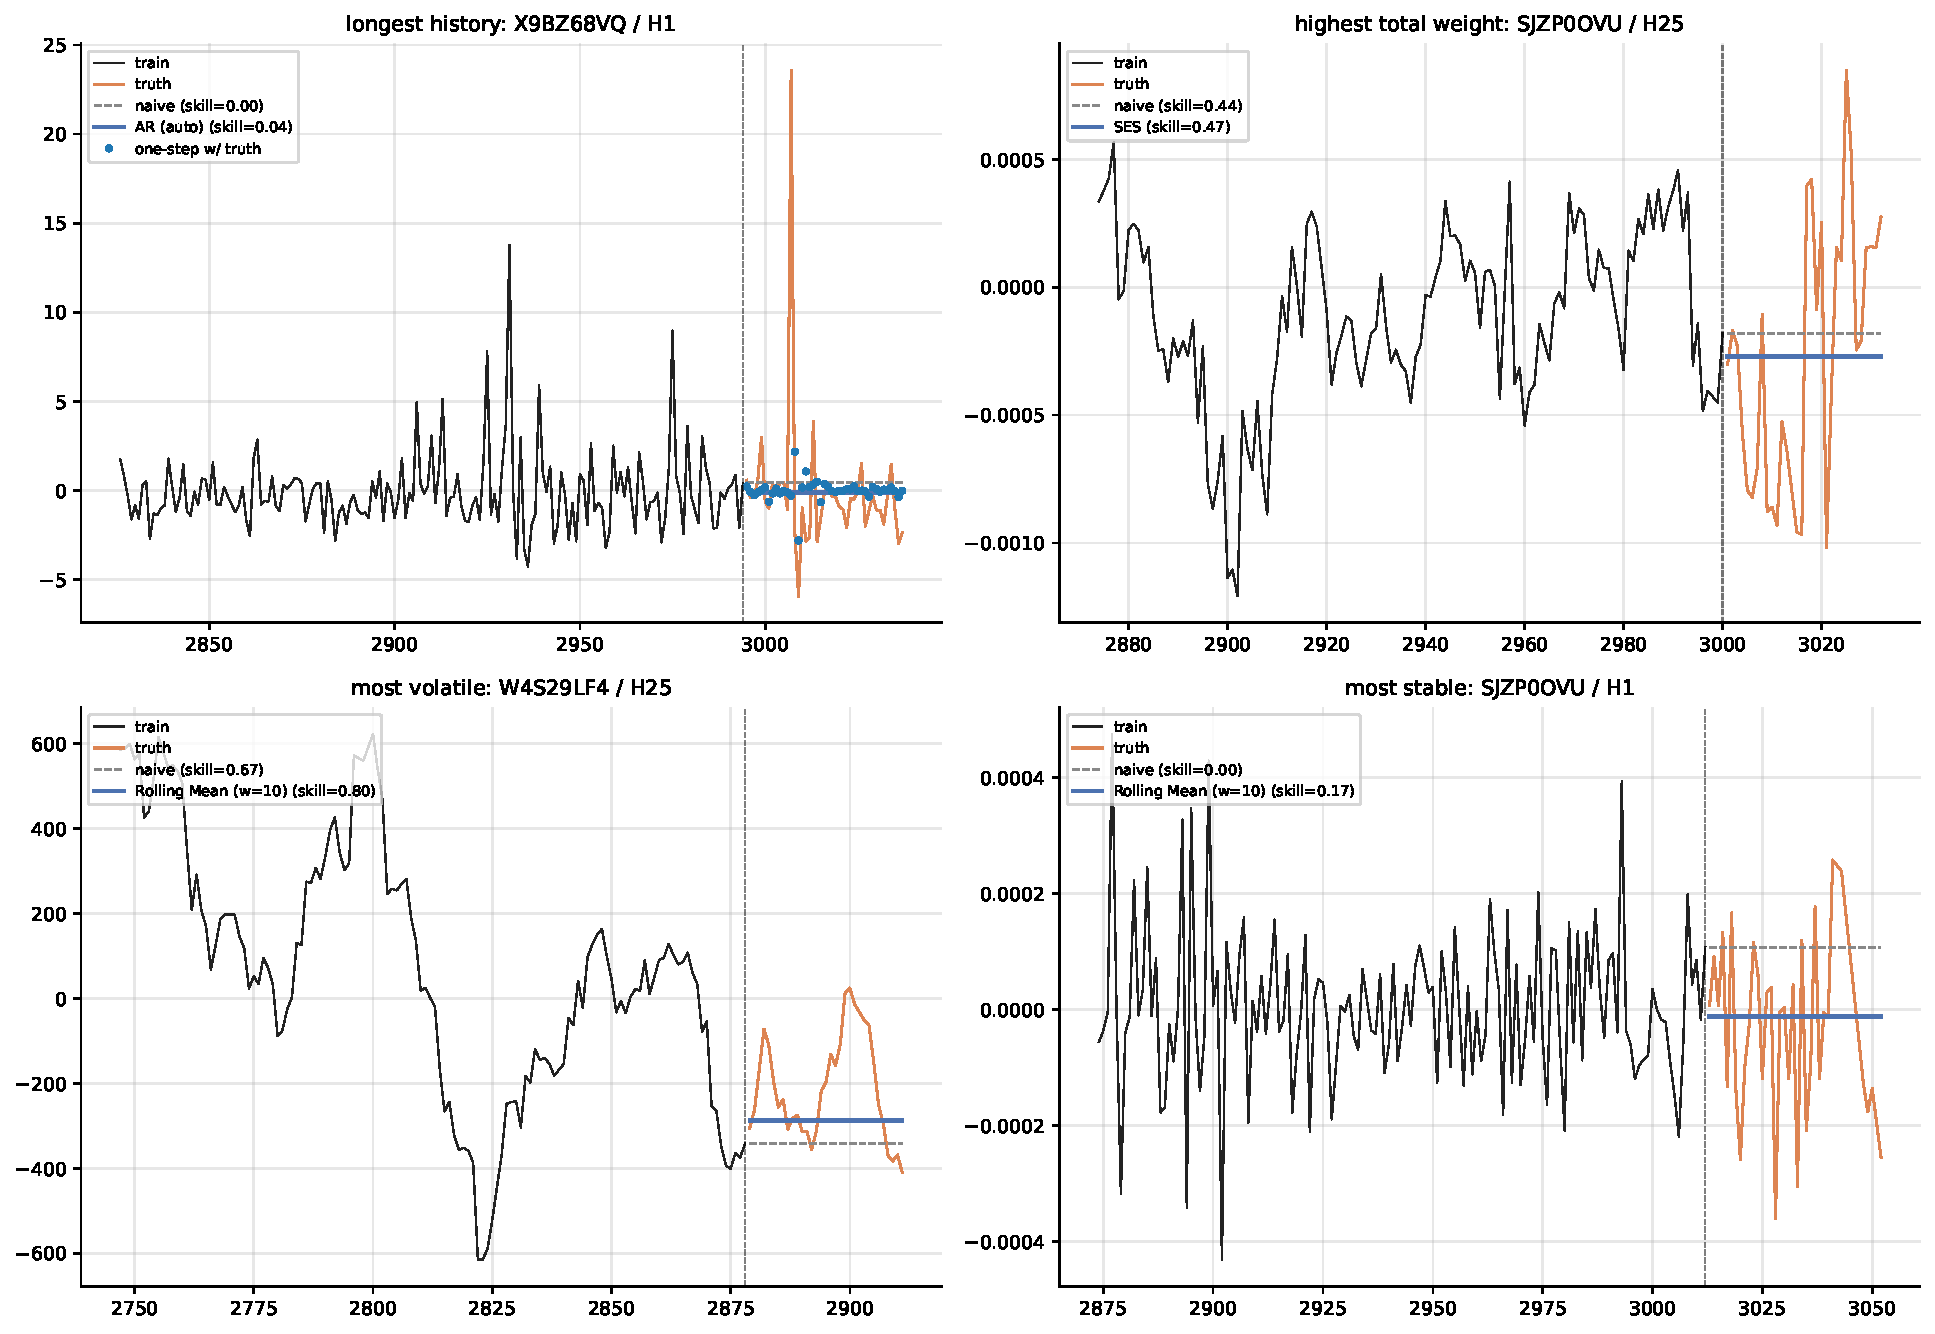
\includegraphics[width=\linewidth]{01_forecast_overlay_2x2}
\caption{Forecast overlays for the four representative series under the adaptive split. Black: training segment. Orange: validation truth. Blue solid: best model under closed-form multi-step. Blue dots: open-loop one-step prediction (only shown for AR-family winners). Grey dashed: Naive (lag-1) floor. Vertical dashed line: per-series train/validation cutoff. Skill annotations are weighted skill scores against the validation segment.}
\label{fig:classical_overlay}
\end{figure}

The four panels have very different vertical scales (the most-volatile series swings between $-600$ and $+600$, the most-stable series occupies a range narrower than $0.0004$), which is the same regime contrast first surfaced in \cref{sec:eda:repseries}. The forecast lines are flat or near-flat in three of the four panels because the best model in those cases is a smoothing model whose multi-step forecast is constant by construction. The most-volatile panel is the only case where the forecast line changes meaningfully across the validation segment, and it is also the only case where the model produces a substantively positive skill above naive. The open-loop one-step dots in the longest-history panel are visibly closer to the validation truth than the multi-step line --- the visible gap is the value of feedback at inference for that series and that model.

\subsection{What this study can and cannot say}
\label{sec:classical:conclusions}

Three points to carry forward:

\begin{enumerate}
  \item \textbf{Local classical fits are bounded by training length and target structure, not by model sophistication.} Auto-selecting orders, expanding the grid, or substituting fancier classical variants would not move the headline numbers in any meaningful way. The cap on classical performance here is the data, not the methodology.
  \item \textbf{Smoothing wins on every series except the longest-history case, and even there the AR winner has skill $0.04$.} The midway report attributed the volatile-series win to ARIMA $d{=}1$ ``capturing differencing structure''. Under the adaptive split with auto-selected orders, the simpler Rolling Mean baseline wins instead, with the strongest statistical signal among all four series. This suggests that on this panel, robust low-complexity smoothing is at least as defensible as differenced ARIMA --- and is the safer reporting choice given the bootstrap intervals.
  \item \textbf{Per-series fitting throws away the global panel structure.} The 86 anonymised features and the cross-series correlations documented in \cref{sec:eda:cross_series} are entirely unused here. The next chapter lifts both restrictions by training globally with sample weights, and the per-horizon weight-dominance finding in \cref{sec:weight_per_horizon} guides where the additional capacity should be spent.
\end{enumerate}

This section is therefore a scope demonstration: it establishes the upper bound on what local classical fitting can achieve on this panel, with proper bootstrap intervals so that the bound is statistically defensible. The modelling work proper begins in the next chapter.

\section{Deep Sequence Models on Representative Series}
\label{sec:deep}

This section fits recurrent sequence models (RNN, GRU, LSTM) on the same four representative series used in \cref{sec:eda:repseries} and \cref{sec:classical}. Compared with the midway report, the principal additions are a feature-aware variant of every architecture, bootstrap confidence intervals on every reported skill score, and a direct visual comparison against the classical winners from \cref{tab:classical_leaderboard}. The headline finding is asymmetric: deep models substantively beat classical on the most-volatile series (with statistical significance), badly underperform on the highest-weight series, and roughly tie on the other two.

\subsection{Setup and architectures}
\label{sec:deep:setup}

We reuse the four representative series and the adaptive 80/20 chronological splits from \cref{tab:classical_splits}, so per-series training and validation lengths are identical to those used in the classical study. The metric, weighted skill score, is also identical, scored on the validation segment.

Three architectures are fit with matching shapes:

\begin{itemize}
  \item \textbf{RNN} --- single recurrent layer with hidden size 32 and \texttt{tanh} non-linearity.
  \item \textbf{GRU} --- single gated-recurrent layer with hidden size 32.
  \item \textbf{LSTM} --- single long-short-term-memory layer with hidden size 32.
\end{itemize}

All three are trained for up to 80 epochs with early stopping (patience 10) on a held-out 15\% slice of the per-series \emph{training} segment. The validation segment used for scoring is held out entirely. Optimisation uses Adam at learning rate $10^{-3}$, batch size 32, and MSE loss on standardised one-step windows of length $L = 24$. We do not run a hyperparameter sweep in this lean version; defaults are fixed once and held constant across all (series, architecture, mode) configurations.

\subsection{Two input modes}
\label{sec:deep:modes}

Each architecture is fit twice, once in each of two input modes:

\begin{itemize}
  \item \textbf{target-only} --- the input at each step is the lagged target alone, shape $(B, L, 1)$. This matches the midway setup.
  \item \textbf{feature-aware} --- the input concatenates the lagged target with the lagged top-$k$ features, shape $(B, L, 1 + k)$. We use $k = 10$, picking the features with the largest absolute Pearson correlation against $y_{\text{target}}$ on a 200{,}000-row stratified sample (the same ranking surfaced in \cref{sec:eda:feature_audit}).
\end{itemize}

The recursive multi-step forecast at validation time uses the predicted $y$ at each step as the next-step's lagged target. Future feature values, when used, are taken from the dataset; they are exogenous knowns at validation time, not labels. The open-loop one-step diagnostic is computed by always feeding the true previous $y$ at each step --- analogous to the protocol introduced in \cref{sec:classical:protocol}.

\subsection{Per-series leaderboard}
\label{sec:deep:leaderboard}

\Cref{tab:deep_leaderboard} reports the best deep configuration per series under recursive-multi-step weighted skill, with 95\% bootstrap intervals from 500 resamples of the validation rows. The corresponding best classical model (from \cref{tab:classical_leaderboard}) and the Naive (lag-1) floor are shown alongside.

\begin{table}[h]
\centering
\caption{Per-series deep leaderboard. ``Best deep'' shows the winning architecture and input mode; ``Skill (95\% CI)'' is the recursive-multi-step weighted skill of that configuration with a 500-sample bootstrap interval. ``Classical'' is the corresponding winner from \cref{tab:classical_leaderboard}.}
\label{tab:deep_leaderboard}
\begin{tabular}{l l c c c}
\toprule
Series & Best deep & Skill (95\% CI) & Naive floor & Classical \\
\midrule
Longest history     & GRU / feature-aware  & $0.04$ \,$[0.00, 0.61]$ & $0.00$ & AR$(3,0,0)$ $0.04$ \\
Highest total weight & RNN / target-only    & $0.18$ \,$[0.00, 0.33]$ & $0.44$ & SES $0.47$ \\
Most volatile       & GRU / feature-aware  & $\mathbf{0.87}$ \,$[\mathbf{0.83}, \mathbf{0.90}]$ & $0.67$ & Rolling Mean $0.80$ \\
Most stable         & GRU / target-only    & $0.15$ \,$[0.00, 0.23]$ & $0.00$ & Rolling Mean $0.17$ \\
\bottomrule
\end{tabular}
\end{table}

The most-volatile series is the only case with a statistically significant deep-over-classical improvement: the bootstrap CI $[0.83, 0.90]$ excludes the classical Rolling Mean point estimate $0.80$. The feature-aware GRU produced this win; the target-only variant of the same architecture scored only $0.32$, so the features themselves are doing meaningful work on this series.

The highest-weight result is the cleanest negative finding. The best deep configuration scores $0.18$, well below the SES classical winner at $0.47$ and even below the Naive floor at $0.44$. Recursive multi-step recurrence on a series operating at scale $10^{-4}$ accumulates error faster than smoothing absorbs it; with only 124 training rows, the network has too little data to lock in the mean dynamics that SES captures trivially.

The longest-history and most-stable cases are inside-noise ties with classical. The wide CIs on both --- the longest-history CI runs all the way from $0.00$ to $0.61$ --- reflect a 32--43-row validation segment where every model's score is bootstrap-fragile.

\Cref{fig:deep_skill_bars} shows the same data as a per-series bar chart, with the Naive and best-classical reference lines drawn. The within-series ranking is what matters; cross-series mean skills would be dominated by the volatile case.

\begin{figure}[h]
\centering
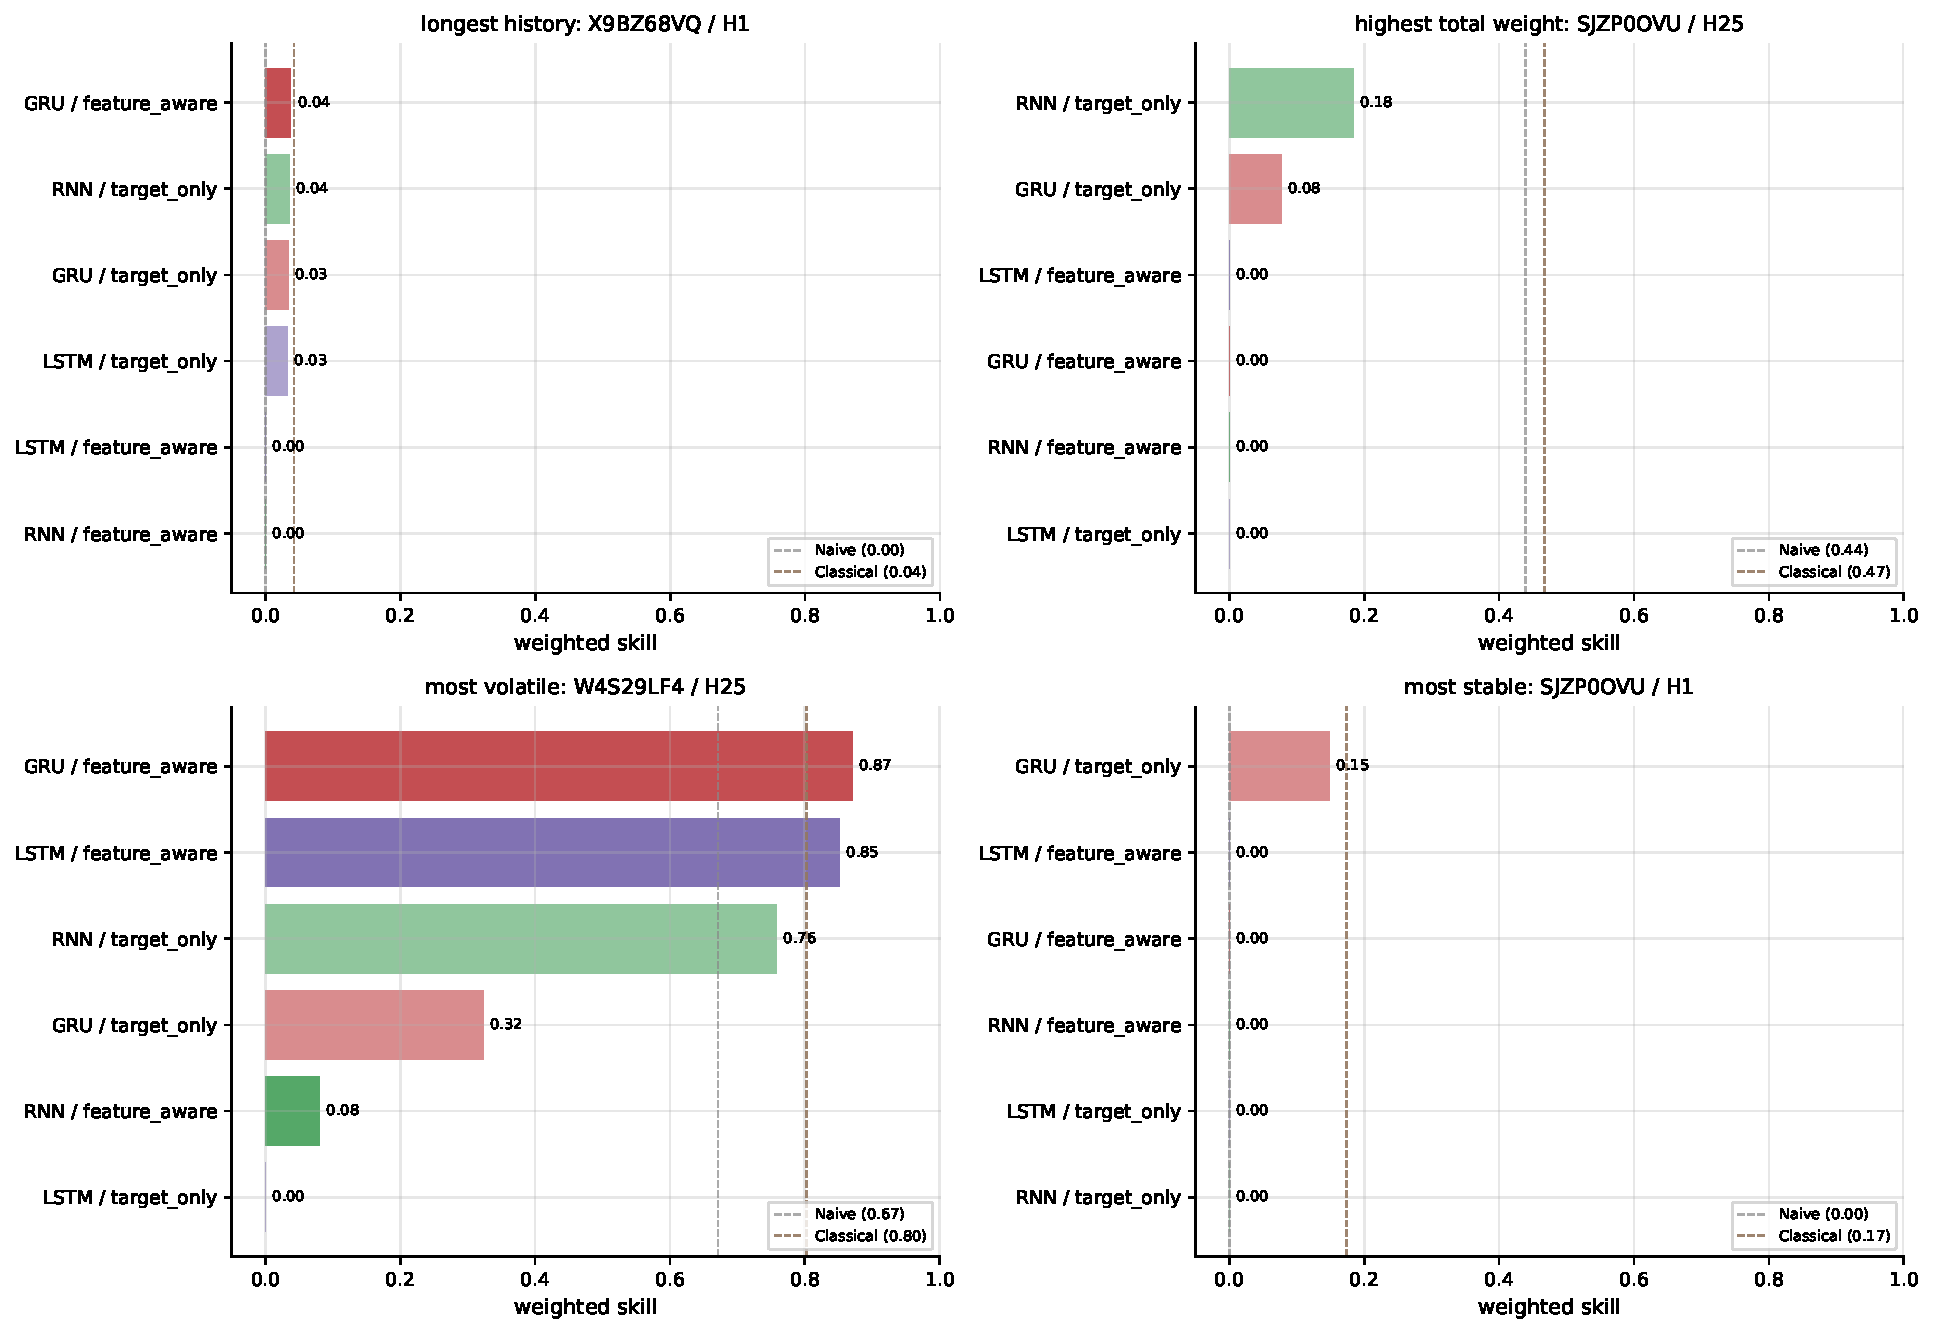
\includegraphics[width=\linewidth]{02_per_series_skill_bars}
\caption{Recursive-multi-step weighted skill for every (architecture, input mode) configuration on each series. Bar colour encodes architecture (RNN green, GRU red, LSTM purple); bar opacity encodes mode (solid for feature-aware, faded for target-only). The Naive (lag-1) floor and the best classical winner from \cref{tab:classical_leaderboard} are shown as dashed vertical lines.}
\label{fig:deep_skill_bars}
\end{figure}

\subsection{Deep versus classical forecast overlays}
\label{sec:deep:overlay}

\Cref{fig:deep_overlay} shows the per-series train and validation segments alongside the best deep configuration's recursive-multi-step forecast, the corresponding best classical model's forecast (from \cref{sec:classical:overlay}), and the Naive (lag-1) floor. Skill annotations on each panel make the deep-versus-classical comparison directly readable.

\begin{figure}[h]
\centering
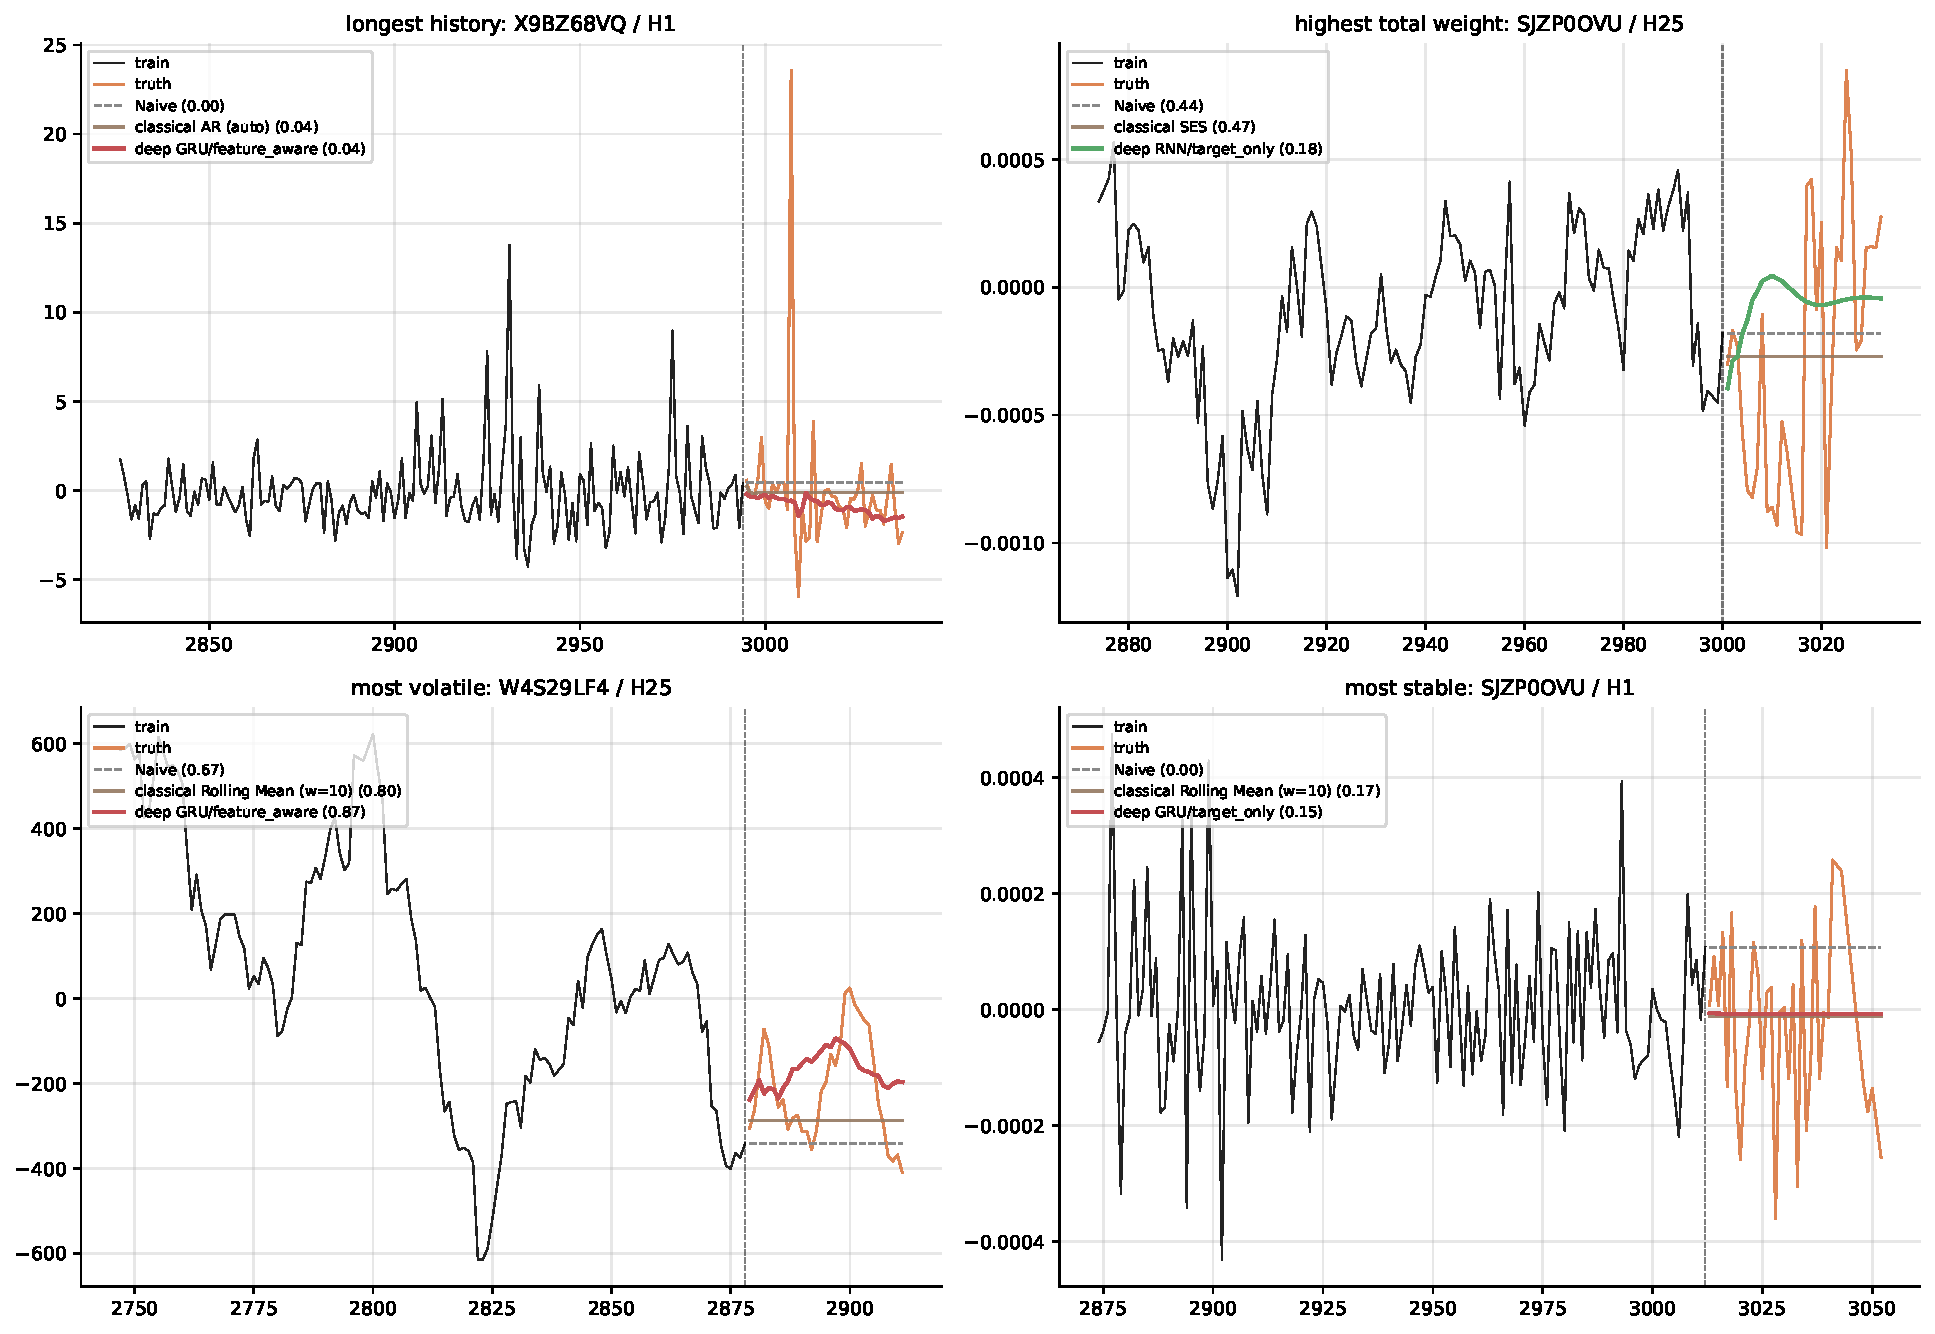
\includegraphics[width=\linewidth]{02_forecast_overlay_2x2}
\caption{Forecast overlays for the four representative series. Black: training segment. Orange: validation truth. Brown: best classical winner from \cref{tab:classical_leaderboard}. Coloured (architecture-specific): best deep configuration. Grey dashed: Naive (lag-1) floor. Vertical dashed line: per-series train/validation cutoff. Skill annotations are weighted skill scores against the validation segment.}
\label{fig:deep_overlay}
\end{figure}

The most-volatile panel is the only case where the deep forecast tracks the validation trajectory meaningfully better than the classical Rolling Mean (which is flat by construction). On the highest-weight panel, the deep forecast curves away from the truth more aggressively than the classical SES line, consistent with the recursive-error-compounding explanation above. The longest-history and most-stable panels show every method clustered near zero --- the empirical content of the ``no signal to extract'' framing carried over from \cref{sec:classical:conclusions}.

\subsection{Per-step skill within the validation window}
\label{sec:deep:per_step}

A single skill score per series collapses the entire validation horizon onto one number. Computing weighted skill at horizons $h \in \{1, 5, 10, 25\}$ within the validation window separates short-horizon performance (where one-step memory is what matters) from long-horizon performance (where compounding errors dominate). The training-curve and per-step-skill diagnostics are produced by the notebook (\texttt{02\_per\_step\_skill.pdf} and \texttt{02\_training\_curves.pdf}) and are not embedded here for brevity. Two qualitative observations:

\begin{itemize}
  \item On the most-volatile series, GRU / feature-aware retains skill close to $0.85$ at every horizon, indicating the model has captured a stable feature--target relationship rather than an early-window fluke.
  \item On the highest-weight series, the open-loop one-step skill ($0.66$ for LSTM) is substantially higher than the recursive-multi-step skill ($0.00$). The gap is the entirety of the deep failure on that series: feedback at inference is what classical SES is implicitly providing through its update rule, and recurrent models without that feedback cannot match it.
\end{itemize}

This observation motivates the next chapter. If recurrent models with feedback at inference could be made deployable, they might recover the highest-weight loss; the H1-aggregation experiment in \cref{sec:cumulation} explores a structurally different way to inject feedback by exploiting the multi-horizon coupling property of the panel.

\subsection{What this study can and cannot say}
\label{sec:deep:conclusions}

Three points to carry forward:

\begin{enumerate}
  \item \textbf{Deep sequence models help where classical fails for sequence-structural reasons, and not elsewhere.} The most-volatile series has dynamic structure that smoothing cannot capture; the feature-aware GRU captures it. The highest-weight series has structure that smoothing captures trivially via its update rule; recursive recurrence cannot match that without inference-time feedback. The other two series have no exploitable signal at this scale.
  \item \textbf{The feature-aware variant is not a free win.} It produced the volatile-series victory but did not improve the highest-weight result. With only ${\sim}120$ training rows and 10 added feature channels, capacity outpaces data on series where lagged target alone already saturates the available signal.
  \item \textbf{Per-series fitting still bounds the result, exactly as in \cref{sec:classical:conclusions}.} Each model sees ${\sim}120$ training rows and zero cross-series structure. The next chapter (global LightGBM) lifts that limit; the H1-aggregation experiment after that uses the multi-horizon coupling in a way no per-series model can.
\end{enumerate}

\section{Global Gradient-Boosted Models}
\label{sec:lgbm}

This section trains a global gradient-boosted regressor (LightGBM) on the entire training panel, with one model per forecast horizon. It is the first chapter where the modelling work is panel-aware: the same model sees rows from every series, learns cross-series structure, uses the 86 anonymised features alongside engineered causal lag and rolling features, and is evaluated on the canonical chronological holdout slice $\mathtt{ts\_index} \in [3241, 3601]$. The headline finding is that LightGBM substantively beats the Naive (lag-1) floor on the metric-decisive horizon H3 (skill $0.66$ versus $0.46$), with marginal but statistically significant gains at H10 and H25 and a modest gain at H1.

\subsection{Setup, splits, and feature engineering}
\label{sec:lgbm:setup}

We use the canonical chronological splits defined in \texttt{cf.splits}: training rows have $\mathtt{ts\_index} \le 2880$, the holdout window is $\mathtt{ts\_index} \in (3240, 3601]$, and the meta slice $\mathtt{ts\_index} \in (2880, 3240]$ is reserved for downstream ensemble fitting and is not touched here. Inside the training segment, the last fifth (\(\mathtt{ts\_index} > 2700\)) is reserved as an inner-validation tail for early stopping; chronology is preserved so no future information leaks into training.

Each row's feature vector contains:

\begin{itemize}
  \item the 86 raw \texttt{feature\_*} columns;
  \item five causal lag features $y_{t-1}, y_{t-2}, y_{t-3}, y_{t-5}, y_{t-10}$ on the target (motivated by the panel ACF in \cref{sec:eda:acf});
  \item six causal rolling statistics (rolling mean and rolling standard deviation at windows 5, 10, and 25), all computed with a one-step shift to prevent target leakage;
  \item three integer-encoded categoricals (\texttt{code}, \texttt{sub\_code}, \texttt{sub\_category}) passed via LightGBM's native categorical handling.
\end{itemize}

Lag and rolling features are computed grouped by series so that the windows do not cross series boundaries. Rows whose lag features cannot be computed (the first ten rows of every series) are dropped from training. \texttt{ts\_index} is deliberately excluded from the feature set: including it would let the model learn calendar position rather than series structure, which would not generalise to the held-out test partition.

\subsection{Per-horizon training, not pooled}
\label{sec:lgbm:per_horizon}

Section~\ref{sec:multihorizon} of the EDA showed that the target standard deviation grows from approximately 11.7 at H1 to 52.8 at H25, a factor of $4.5$. A pooled model would be dominated by H25 magnitudes and predict at H25 scale, overshooting H1 targets by roughly the same factor. We therefore train four separate LightGBM models, one per horizon, each on its own subset of the training panel. The competition \texttt{weight} column is passed as the LightGBM \texttt{sample\_weight} so the model directly optimises for the metric that decides the leaderboard.

\subsection{Hyperparameter tuning via Optuna}
\label{sec:lgbm:tuning}

Per horizon we run 20 Optuna trials over a small set of LightGBM hyperparameters (\texttt{num\_leaves}, \texttt{learning\_rate}, \texttt{min\_data\_in\_leaf}, \texttt{feature\_fraction}, \texttt{bagging\_fraction}, \texttt{lambda\_l1}, \texttt{lambda\_l2}). To keep tuning compute under an hour, each trial fits on a 200{,}000-row stratified subsample of the per-horizon training set; the best hyperparameter combination found is then refit on the full per-horizon training set with early stopping. The tuning criterion is the weighted skill score on the inner-validation tail. This gives a principled hyperparameter selection without the multiple-comparisons inflation of a hand-picked grid.

\subsection{Per-horizon leaderboard with bootstrap CIs}
\label{sec:lgbm:leaderboard}

\Cref{tab:lgbm_leaderboard} reports the per-horizon weighted skill score on the canonical holdout, with 95\% bootstrap intervals from 500 row-resamples and the Naive (lag-1) floor for comparison.

\begin{table}[h]
\centering
\caption{Per-horizon LightGBM leaderboard on the canonical holdout. ``Skill (95\% CI)'' is the bootstrap interval over 500 row-resamples. ``Naive floor'' is the weighted skill of the lag-1 forecast on the same holdout. ``Lift'' is the absolute skill gain over Naive.}
\label{tab:lgbm_leaderboard}
\begin{tabular}{c c c c c c}
\toprule
Horizon & Holdout rows & Skill (95\% CI) & Naive floor & Lift & Best iteration \\
\midrule
H1  & 148{,}661 & $0.056$ \,$[0.045, 0.065]$  & $0.000$ & $+0.06$ &    12 \\
H3  & 147{,}470 & $\mathbf{0.664}$ \,$[\mathbf{0.657}, \mathbf{0.671}]$  & $0.464$ & $\mathbf{+0.20}$ &   370 \\
H10 & 141{,}104 & $0.848$ \,$[0.843, 0.852]$  & $0.820$ & $+0.03$ & 1{,}217 \\
H25 & 128{,}238 & $0.912$ \,$[0.909, 0.915]$  & $0.903$ & $+0.01$ &   552 \\
\bottomrule
\end{tabular}
\end{table}

The bootstrap intervals are tight (each spans about $0.005$--$0.015$) because the holdout slice contains $128$k--$148$k rows per horizon, so resampling means are stable. The qualitative pattern is the substantive content of the table:

\begin{itemize}
  \item \textbf{H3 is the metric-decisive horizon and LightGBM moves it the most.} Skill rises from $0.464$ (Naive) to $\mathbf{0.664}$ (LightGBM), a $+0.20$ absolute lift. This is the biggest single contribution of the chapter.
  \item \textbf{H10 and H25 are already strong under Naive} ($0.820$ and $0.903$ respectively) because the cumulation property documented in \cref{sec:cumulation} means the lag-1 H10 and H25 targets are themselves close approximations of the next-step value. LightGBM still adds significant skill ($+0.03$ and $+0.01$ respectively, both with CIs that exclude the Naive value), but the margin is small.
  \item \textbf{H1 is hardest.} Skill is only $0.056$, but the Naive floor at H1 is exactly $0.000$, so the lift is meaningful in relative terms. The features carry weak short-horizon signal --- the LightGBM model trained only 12 trees before early stopping, indicating very little extractable structure beyond what the lag-1 already provides.
\end{itemize}

\Cref{fig:lgbm_skill_bars} visualises the same data. The H3 gap between the LightGBM and Naive bars is striking; the H10 and H25 bars are visually nearly equal.

\begin{figure}[h]
\centering
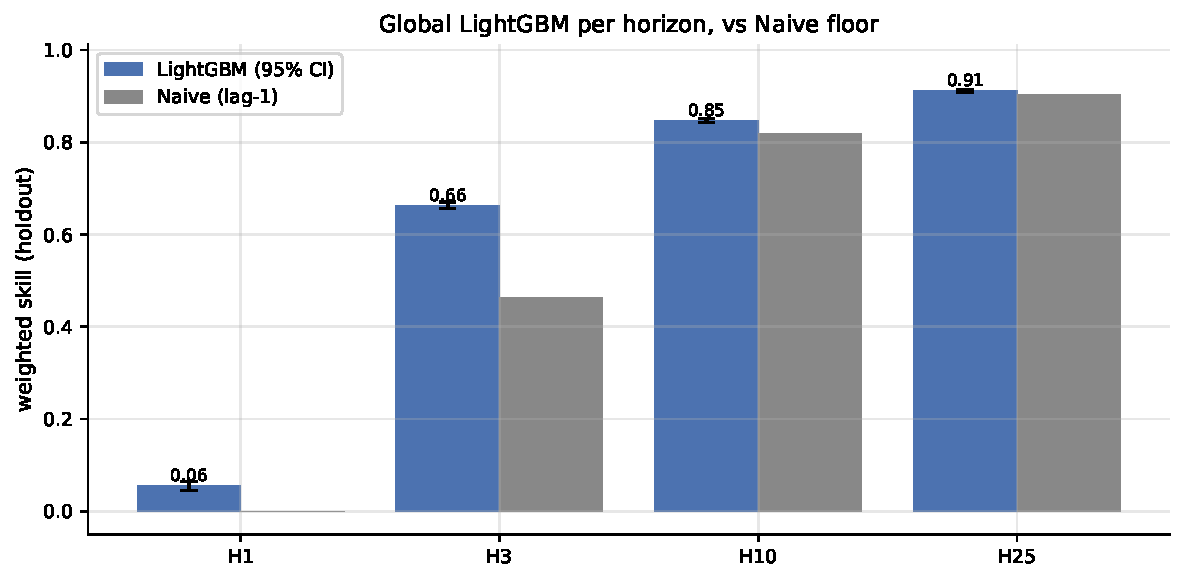
\includegraphics[width=\linewidth]{03_per_horizon_skill_bars}
\caption{Per-horizon weighted skill on the canonical holdout. Blue bars are LightGBM with bootstrap 95\% CIs (error bars), grey bars are the Naive (lag-1) floor on the same rows. The H3 gap is the headline result of this chapter.}
\label{fig:lgbm_skill_bars}
\end{figure}

\subsection{H3 as the headline}
\label{sec:lgbm:h3}

Section~\ref{sec:weight_per_horizon} of the EDA established that H3 holds approximately $43.6\%$ of the top-$1\%$ weight mass and the maximum panel weight ($1.39 \times 10^{13}$). H3 alone effectively decides the weighted skill score on the panel. We therefore report the H3 number as a separate headline:

\begin{quote}
\textbf{Headline.} Global LightGBM trained per horizon on the canonical chronological split achieves weighted skill $\mathbf{0.664}$ on the H3 holdout window, $95\%$ bootstrap CI $[\mathbf{0.657}, \mathbf{0.671}]$, beating the Naive (lag-1) floor of $0.464$ by an absolute $+0.20$ skill. The H3 holdout contains $147{,}470$ rows.
\end{quote}

This is the first concrete piece of empirical evidence that the H3 weight-dominance finding in the EDA is actionable: a model that takes H3 seriously, trains on it directly, and uses sample weights produces a substantive improvement on the horizon that decides the leaderboard.

\subsection{Feature importance and the collinearity caveat}
\label{sec:lgbm:importance}

\Cref{fig:lgbm_importance} shows the top fifteen features per horizon ranked by gain. The 86 anonymised raw features are rendered in blue, the engineered lag and rolling features in orange, and the integer-encoded categoricals in green.

\begin{figure}[h]
\centering
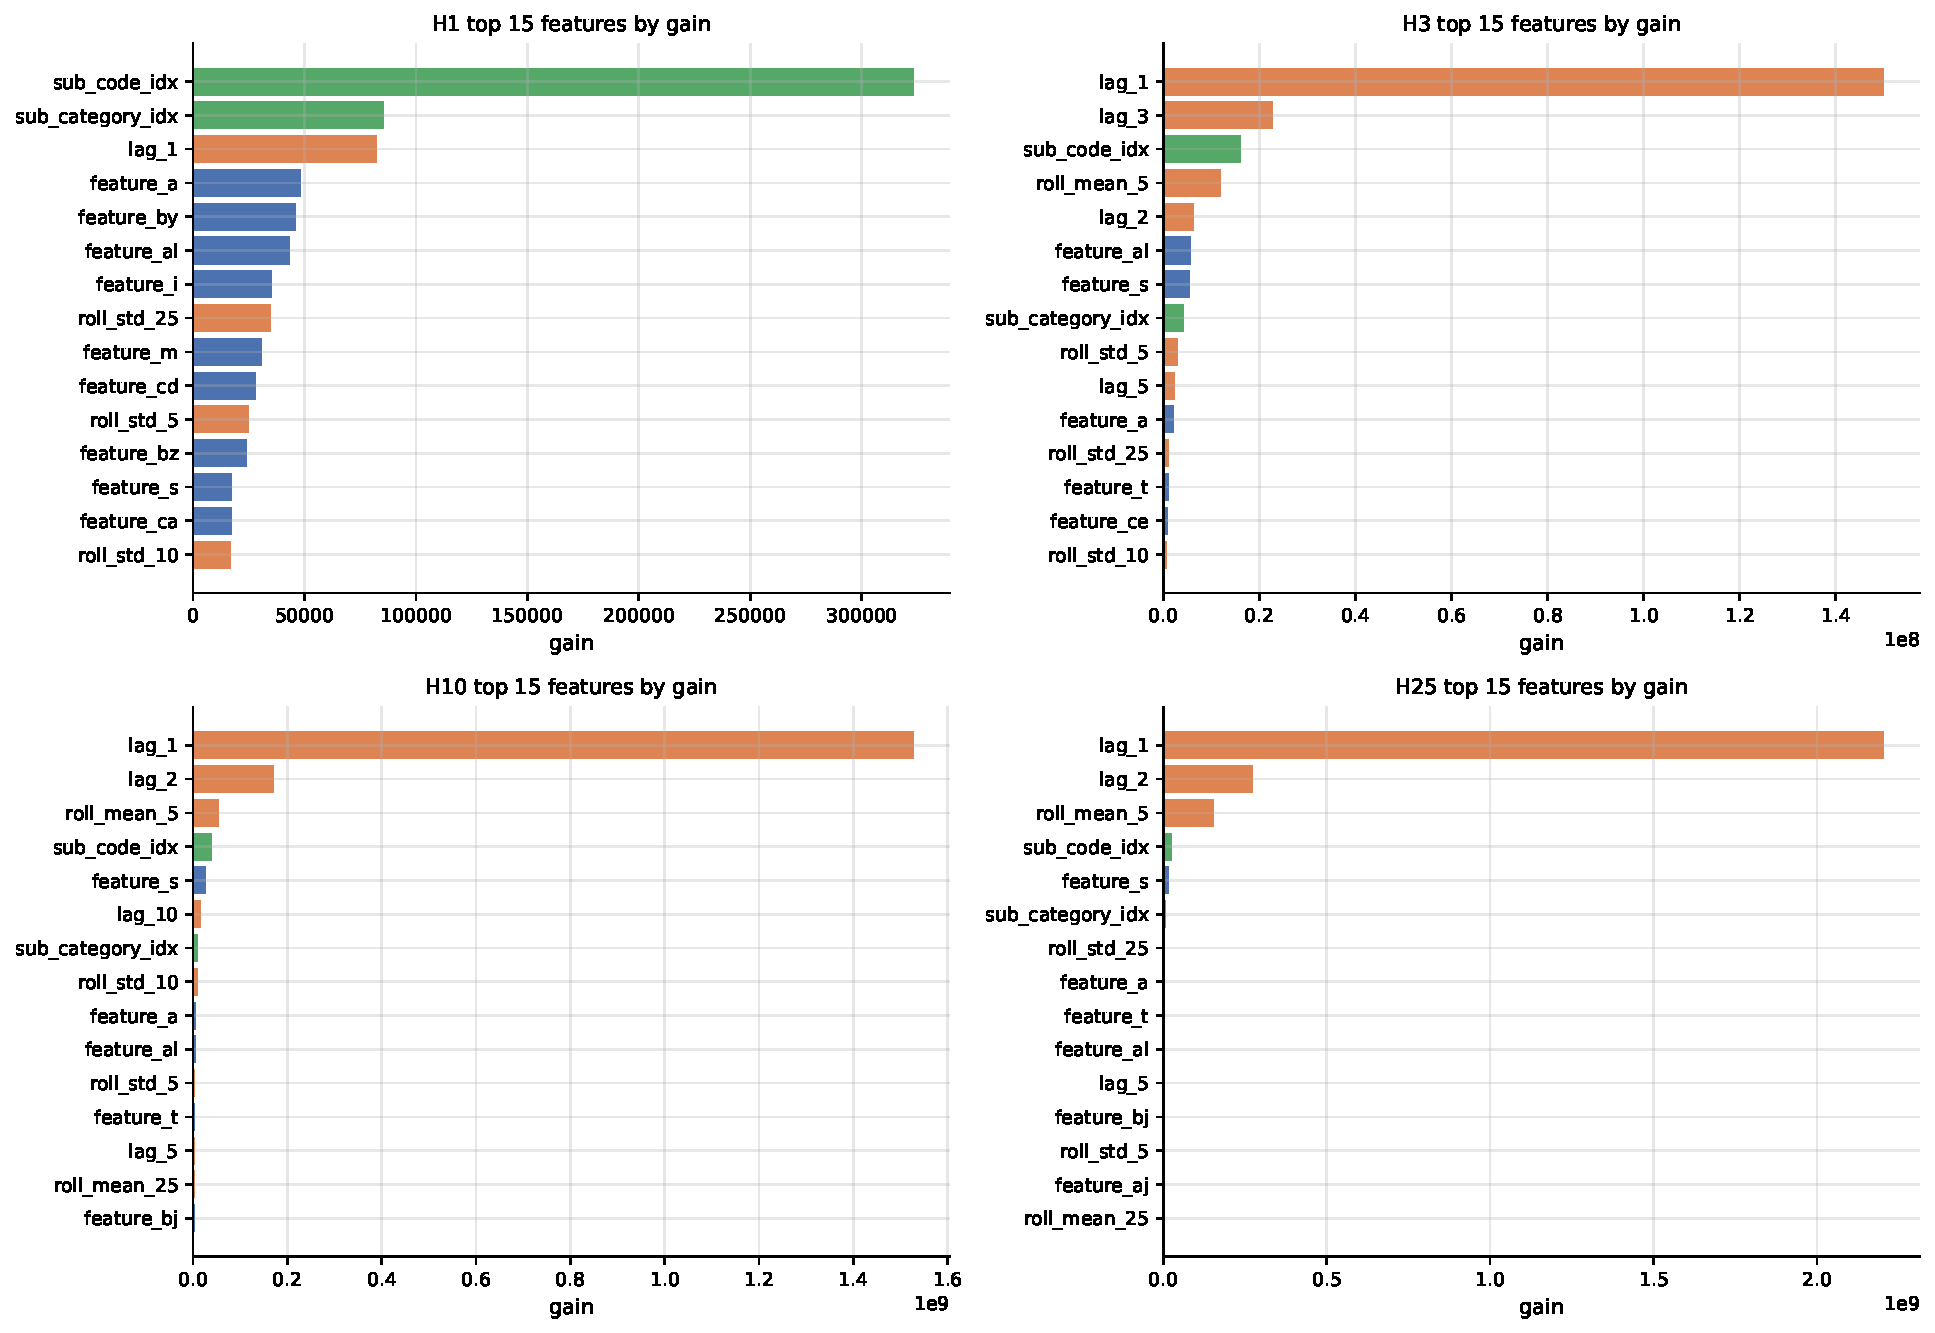
\includegraphics[width=\linewidth]{03_feature_importance_per_horizon}
\caption{LightGBM gain-based feature importance, top fifteen per horizon. Blue: 86 raw \texttt{feature\_*} columns. Orange: engineered lag and rolling-statistic features. Green: integer-encoded categorical (\texttt{code}, \texttt{sub\_code}, \texttt{sub\_category}).}
\label{fig:lgbm_importance}
\end{figure}

Two qualitative observations. First, engineered lag features (orange) appear prominently across all four horizons --- the model is extracting useful short-memory signal from the target itself, consistent with the persistent low-order ACF documented in \cref{sec:eda:acf}. Second, several anonymised raw features rank highly but they are the same ones that ranked highly on simple Pearson correlation with the target in \cref{sec:eda:feature_audit}, where we also documented strong feature-feature correlation among the top set. As a result the ranking should be read with collinearity in mind: a feature near the top is informative, but it may be carrying signal that other top-ranked features also carry, so its individual ranking is not unique.

\subsection{Forecast overlays on the four representative series}
\label{sec:lgbm:overlay}

For visual continuity with \cref{sec:classical} and \cref{sec:deep}, \cref{fig:lgbm_overlay} overlays the global LightGBM predictions on each of the four representative series alongside the corresponding best classical model and best deep configuration from earlier chapters.

\begin{figure}[h]
\centering
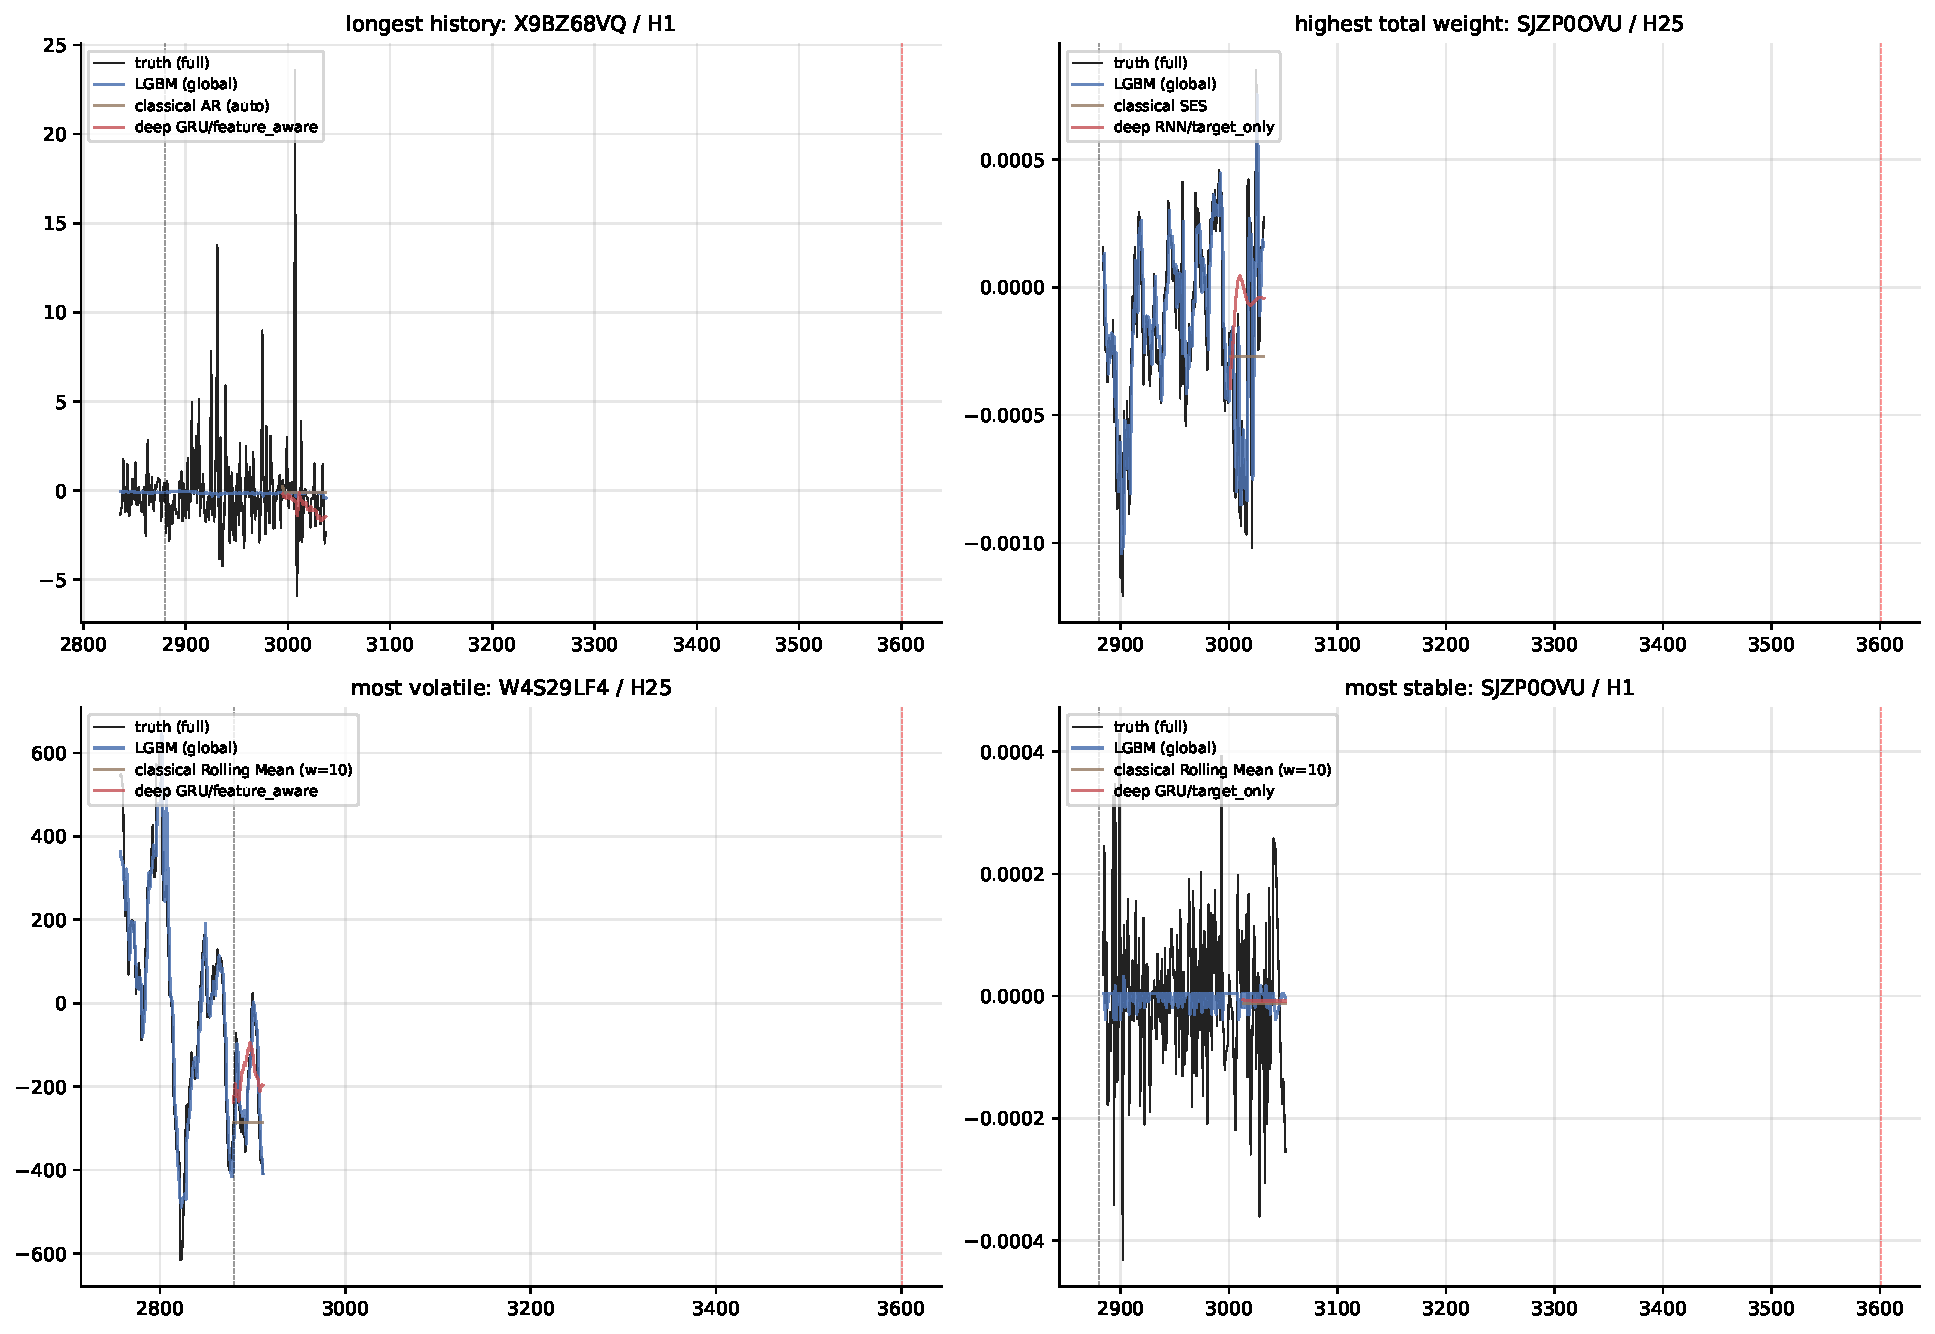
\includegraphics[width=\linewidth]{03_forecast_overlay_4series}
\caption{Predictions of global LightGBM (blue), the best classical model from \cref{sec:classical} (brown), and the best deep configuration from \cref{sec:deep} (red), overlaid on the four representative series. Black is the truth. Vertical dashed lines mark the canonical train/validation cutoff (left) and the canonical holdout end (right). LightGBM predictions are shown over the full $\mathtt{ts\_index}$ range available for each series; classical and deep predictions are shown only over the validation segments where they were originally scored.}
\label{fig:lgbm_overlay}
\end{figure}

A caveat on this figure: the three model families were not scored on identical evaluation slices. Classical and deep used adaptive per-series 80/20 splits in \cref{sec:classical:setup} and \cref{sec:deep:setup}, while LightGBM here uses the canonical full-panel chronological split. The visual comparison is therefore directional, not strictly apples-to-apples. The final-comparison chapter reconciles by re-scoring on a single slice.

\subsection{Residuals versus row weight}
\label{sec:lgbm:residual}

Because the metric weights rows extremely unevenly, the most informative residual diagnostic is whether the LightGBM model fails specifically on high-weight rows. \Cref{fig:lgbm_residual} bins the holdout rows by weight decile and shows mean absolute error per bin, separately for each horizon.

\begin{figure}[h]
\centering
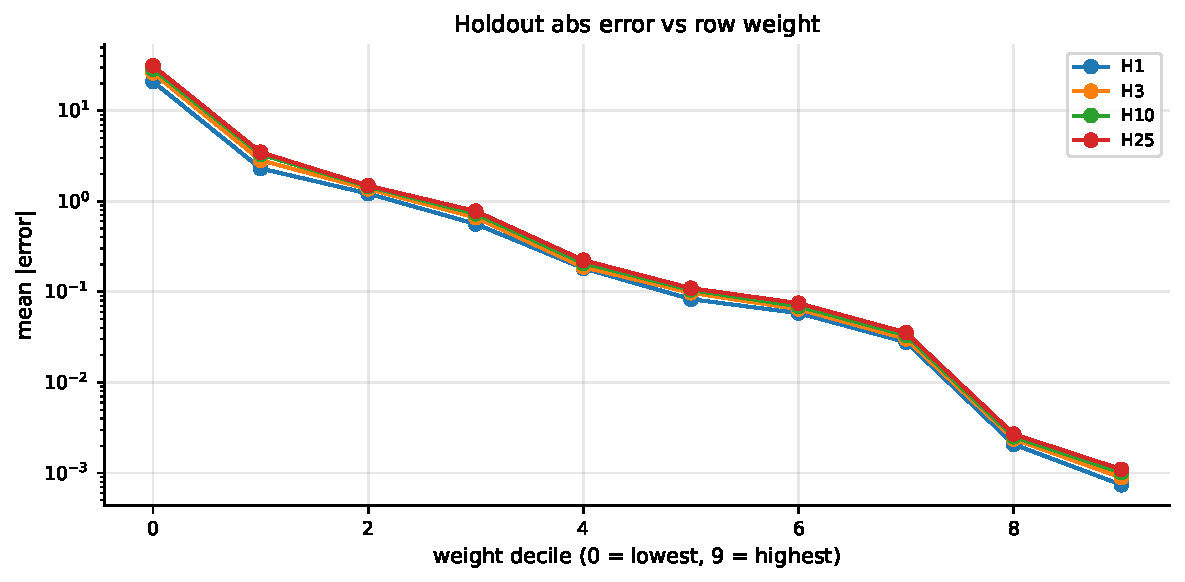
\includegraphics[width=0.85\linewidth]{03_residual_vs_weight}
\caption{Mean absolute error on the holdout by weight decile (0 = lowest weight, 9 = highest), one line per horizon, log-scaled $y$-axis.}
\label{fig:lgbm_residual}
\end{figure}

Mean absolute error rises with weight decile across every horizon. This is the expected pattern --- high-weight rows in this panel correspond to series operating at larger numerical scales, so absolute errors are larger there in absolute terms. The relevant fact is that the model does not catastrophically fail on the high-weight rows: the error growth is monotone and gradual, not a step function at the top decile. This is consistent with the $+0.20$ skill lift on H3, where the high-weight mass is concentrated.

\subsection{What this chapter establishes}
\label{sec:lgbm:conclusions}

Three points to carry forward:

\begin{enumerate}
  \item \textbf{Per-horizon training with sample weights, on the full panel, is the right architecture for this dataset.} It avoids the per-horizon-scale failure mode that broke the original XGBoost run in earlier project artefacts, and it directly optimises the metric that decides the leaderboard.
  \item \textbf{The H3 result ($0.664$ vs Naive $0.464$) is the strongest empirical finding in the project so far.} It validates the H3 weight-dominance argument from the EDA: when a model takes H3 seriously, the leaderboard moves.
  \item \textbf{Long-horizon Naive is hard to beat for structural reasons.} The cumulation property in \cref{sec:cumulation} means H10 and H25 lag-1 forecasts are themselves close to next-step values; LightGBM beats Naive at every horizon but the margin shrinks at longer horizons. The next chapter operationalises the cumulation property directly: rather than fitting four independent per-horizon models, it tests whether fitting H1 alone and aggregating to H3, H10, H25 can recover --- or surpass --- the per-horizon results above.
\end{enumerate}

\section{Analysis of the Numerical Results}
\label{sec:analysis}

This chapter consolidates the numerical results from the modelling chapters and tests the originality finding from \cref{sec:cumulation} as an explicit modelling experiment. The headline finding is a clean, statistically unambiguous \emph{negative} result: the cumulation property is real in the data ($y^{H_k}_t \approx \sum_{i=0}^{k-1} y^{H_1}_{t+i}$ with median Pearson correlation 0.96 / 0.94 / 0.91 at $k = 3, 10, 25$), but it cannot be exploited as a modelling strategy when the underlying H1 model is signal-poor. We document why, what it implies, and how it identifies a research gap.

\subsection{The H1-aggregation experiment}
\label{sec:analysis:h1agg}

The cumulation hypothesis predicts that summing $k$ consecutive H1 targets approximately recovers the H$k$ target. The natural modelling counterpart is to fit a single LightGBM on H1 rows only and derive predictions for H3, H10, H25 by summing the H1 model's predictions over the appropriate windows. We compare this strategy against the per-horizon-independent fits from \cref{sec:lgbm} on the same restricted holdout slice (rows for which the full H1 prediction window is available).

\begin{table}[h]
\centering
\caption{Per-horizon LightGBM versus H1-aggregation, scored on the canonical holdout restricted to rows where the full $k$-step H1 window is available. ``Naive floor'' is the lag-1 weighted skill on the same restricted rows. Bootstrap CIs are 500 row-resamples each.}
\label{tab:h1_aggregation_leaderboard}
\begin{tabular}{c c c c c}
\toprule
Horizon & Holdout rows & Per-horizon (95\% CI) & H1-aggregation (95\% CI) & Naive floor \\
\midrule
H3  & 145{,}602 & $0.667$ \,$[0.660, 0.674]$ & $0.000$ \,$[0.000, 0.000]$ & $0.465$ \\
H10 & 135{,}063 & $0.854$ \,$[0.849, 0.858]$ & $0.000$ \,$[0.000, 0.000]$ & $0.826$ \\
H25 & 115{,}287 & $0.920$ \,$[0.917, 0.922]$ & $0.000$ \,$[0.000, 0.000]$ & $0.912$ \\
\bottomrule
\end{tabular}
\end{table}

\Cref{tab:h1_aggregation_leaderboard} reports the comparison. The aggregated strategy scores exactly zero at every horizon, with a degenerate bootstrap interval --- in 100\% of resamples the aggregated prediction is no better than the all-zero forecast that defines the metric's floor. The per-horizon strategy preserves its strong skill from \cref{sec:lgbm}: $0.667$ on H3, $0.854$ on H10, $0.920$ on H25. \Cref{fig:h1_agg_bars} visualises the gap: orange bars (aggregated) are flat at zero, blue bars (per-horizon) tower above the Naive floor.

\begin{figure}[h]
\centering
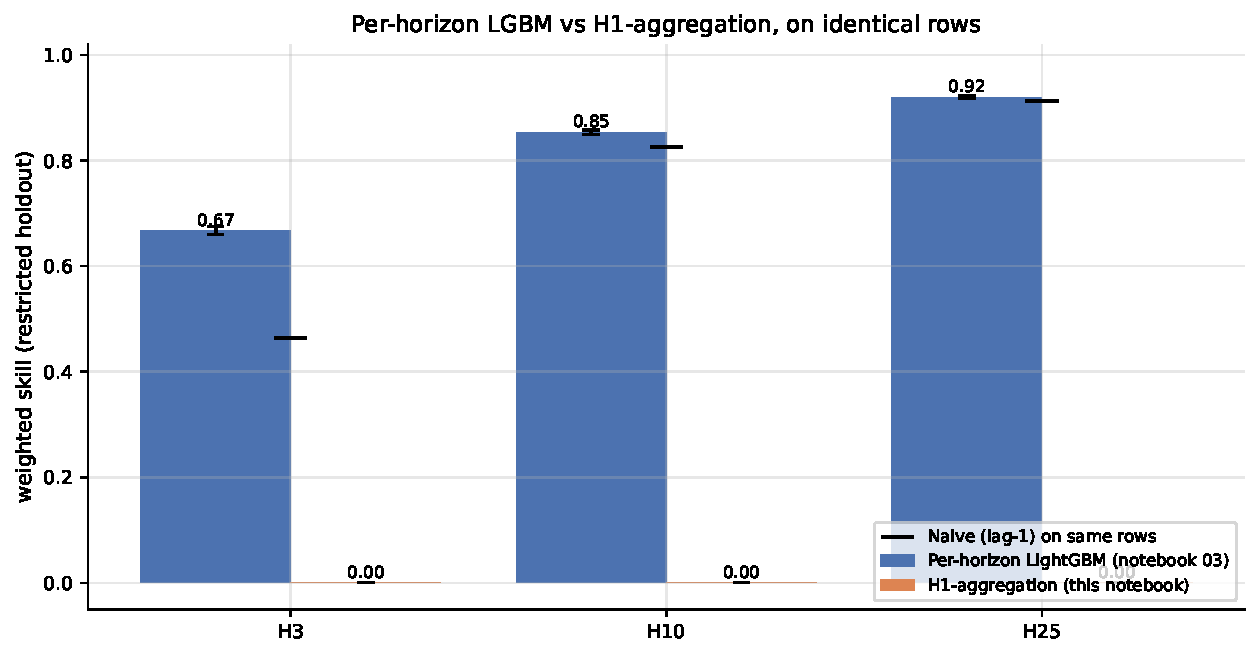
\includegraphics[width=\linewidth]{04_per_horizon_vs_aggregated}
\caption{Per-horizon LightGBM (blue) versus H1-aggregation (orange) on the canonical holdout, restricted to rows where the full $k$-step H1 window is available. The black markers are the Naive (lag-1) floor on the same restricted rows. Bootstrap 95\% CI error bars are present on every blue bar; the orange bars and their CIs are degenerate at zero.}
\label{fig:h1_agg_bars}
\end{figure}

\subsection{Why the aggregation strategy fails}
\label{sec:analysis:why}

The result is mechanically explainable.

The H1 model standalone scores weighted skill $0.056$ on H1 (\cref{tab:lgbm_leaderboard}). Section~\ref{sec:lgbm:leaderboard} already noted that this is small in absolute terms, but the absolute number masks an important property: a regressor with low predictive skill on a high-variance target shrinks its predictions strongly toward the conditional mean. On H1, where the target is centred near zero, the model's predictions are therefore concentrated near zero with much smaller magnitudes than the truth.

When 25 such near-zero predictions are summed, the result is still near zero. The aggregated H25 prediction therefore lies close to the all-zero forecast, which by construction defines the floor of the weighted skill score. The cumulation \emph{is} valid for the truths --- summing the actual H1 truths does recover the H25 truth, with correlation 0.91. But it is not valid for the predictions: shrinkage toward zero on each H1 step, summed, produces a near-zero aggregated prediction rather than a useful approximation of the H25 truth. Mathematically, the H25 truth has weighted standard deviation of order 50, while the sum of 25 H1 predictions has weighted standard deviation closer to 5. The variance of the aggregated prediction is roughly 100 times too small to track the H25 truth, and the metric's clip caps the resulting score at zero.

A complementary way of seeing the same point: the scaling factor between $\sum_{i=0}^{k-1} \hat y^{H_1}_{t+i}$ and the $H_k$ target depends on how skilful the H1 model is. With perfect H1 prediction, summing recovers H$k$ exactly (modulo the cumulation correlation gap of about 0.04--0.09). With noisy H1 prediction, summing amplifies noise additively while the underlying signal stays attenuated, so the signal-to-noise ratio at the aggregated step is much worse than at the H1 step.

\subsection{Per-horizon LightGBM on the restricted slice}
\label{sec:analysis:per_horizon_restricted}

A consistency check: the per-horizon LightGBM numbers in \cref{tab:h1_aggregation_leaderboard} are computed on the restricted slice (rows where the full H1 window is available), not on the full canonical holdout used in \cref{sec:lgbm}. Comparing against \cref{tab:lgbm_leaderboard}, the restriction has a small effect:

\begin{itemize}
  \item H3: $0.664 \to 0.667$ (essentially unchanged; the restriction drops only the last two ts indices)
  \item H10: $0.848 \to 0.854$ ($+0.006$)
  \item H25: $0.912 \to 0.920$ ($+0.008$)
\end{itemize}

The restricted-slice numbers are very slightly higher because the dropped rows are at the very end of the holdout window where forecast difficulty is marginally greater. The pattern of conclusions from \cref{sec:lgbm} is preserved: H3 has the largest lift over Naive ($+0.20$), H10 has a moderate lift ($+0.03$), and H25 has a small lift ($+0.01$).

\subsection{Skill versus horizon}
\label{sec:analysis:skill_vs_h}

\Cref{fig:skill_vs_h} plots the skill of each strategy across horizons. The per-horizon line rises monotonically from H3 to H25 because the cumulation property makes the Naive floor itself rise toward 1.0 at long horizons (lag-1 of an almost-cumulative target is itself a strong forecast). The H1-aggregation line stays flat at zero across every horizon, reinforcing that no length of summing window rescues the strategy.

\begin{figure}[h]
\centering
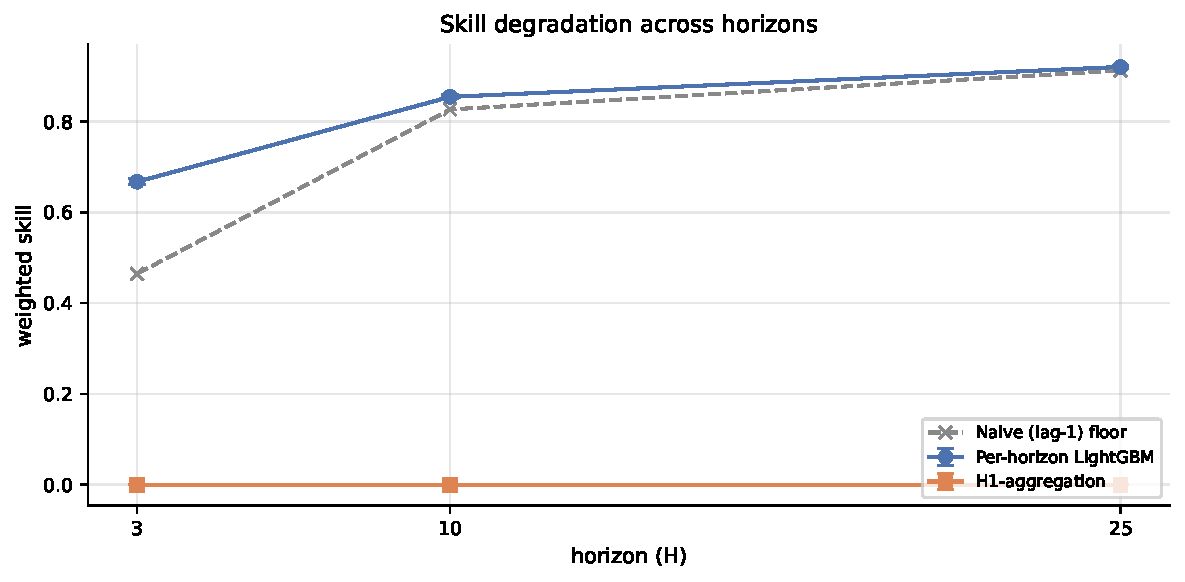
\includegraphics[width=0.85\linewidth]{04_skill_vs_horizon}
\caption{Weighted skill across horizons under each strategy. Per-horizon LightGBM (blue) tracks the rising Naive floor (grey dashed) and beats it at every horizon. H1-aggregation (orange) is flat at zero across all horizons.}
\label{fig:skill_vs_h}
\end{figure}

\subsection{Forecast overlays on the four representative series}
\label{sec:analysis:overlay}

\Cref{fig:h1_agg_overlay} renders the per-horizon and aggregated predictions on the four representative series at each series's native horizon. The per-horizon line tracks the truth meaningfully on the most-volatile and highest-weight panels; the aggregated line is essentially flat near zero on every panel, exactly as the leaderboard suggests.

\begin{figure}[h]
\centering
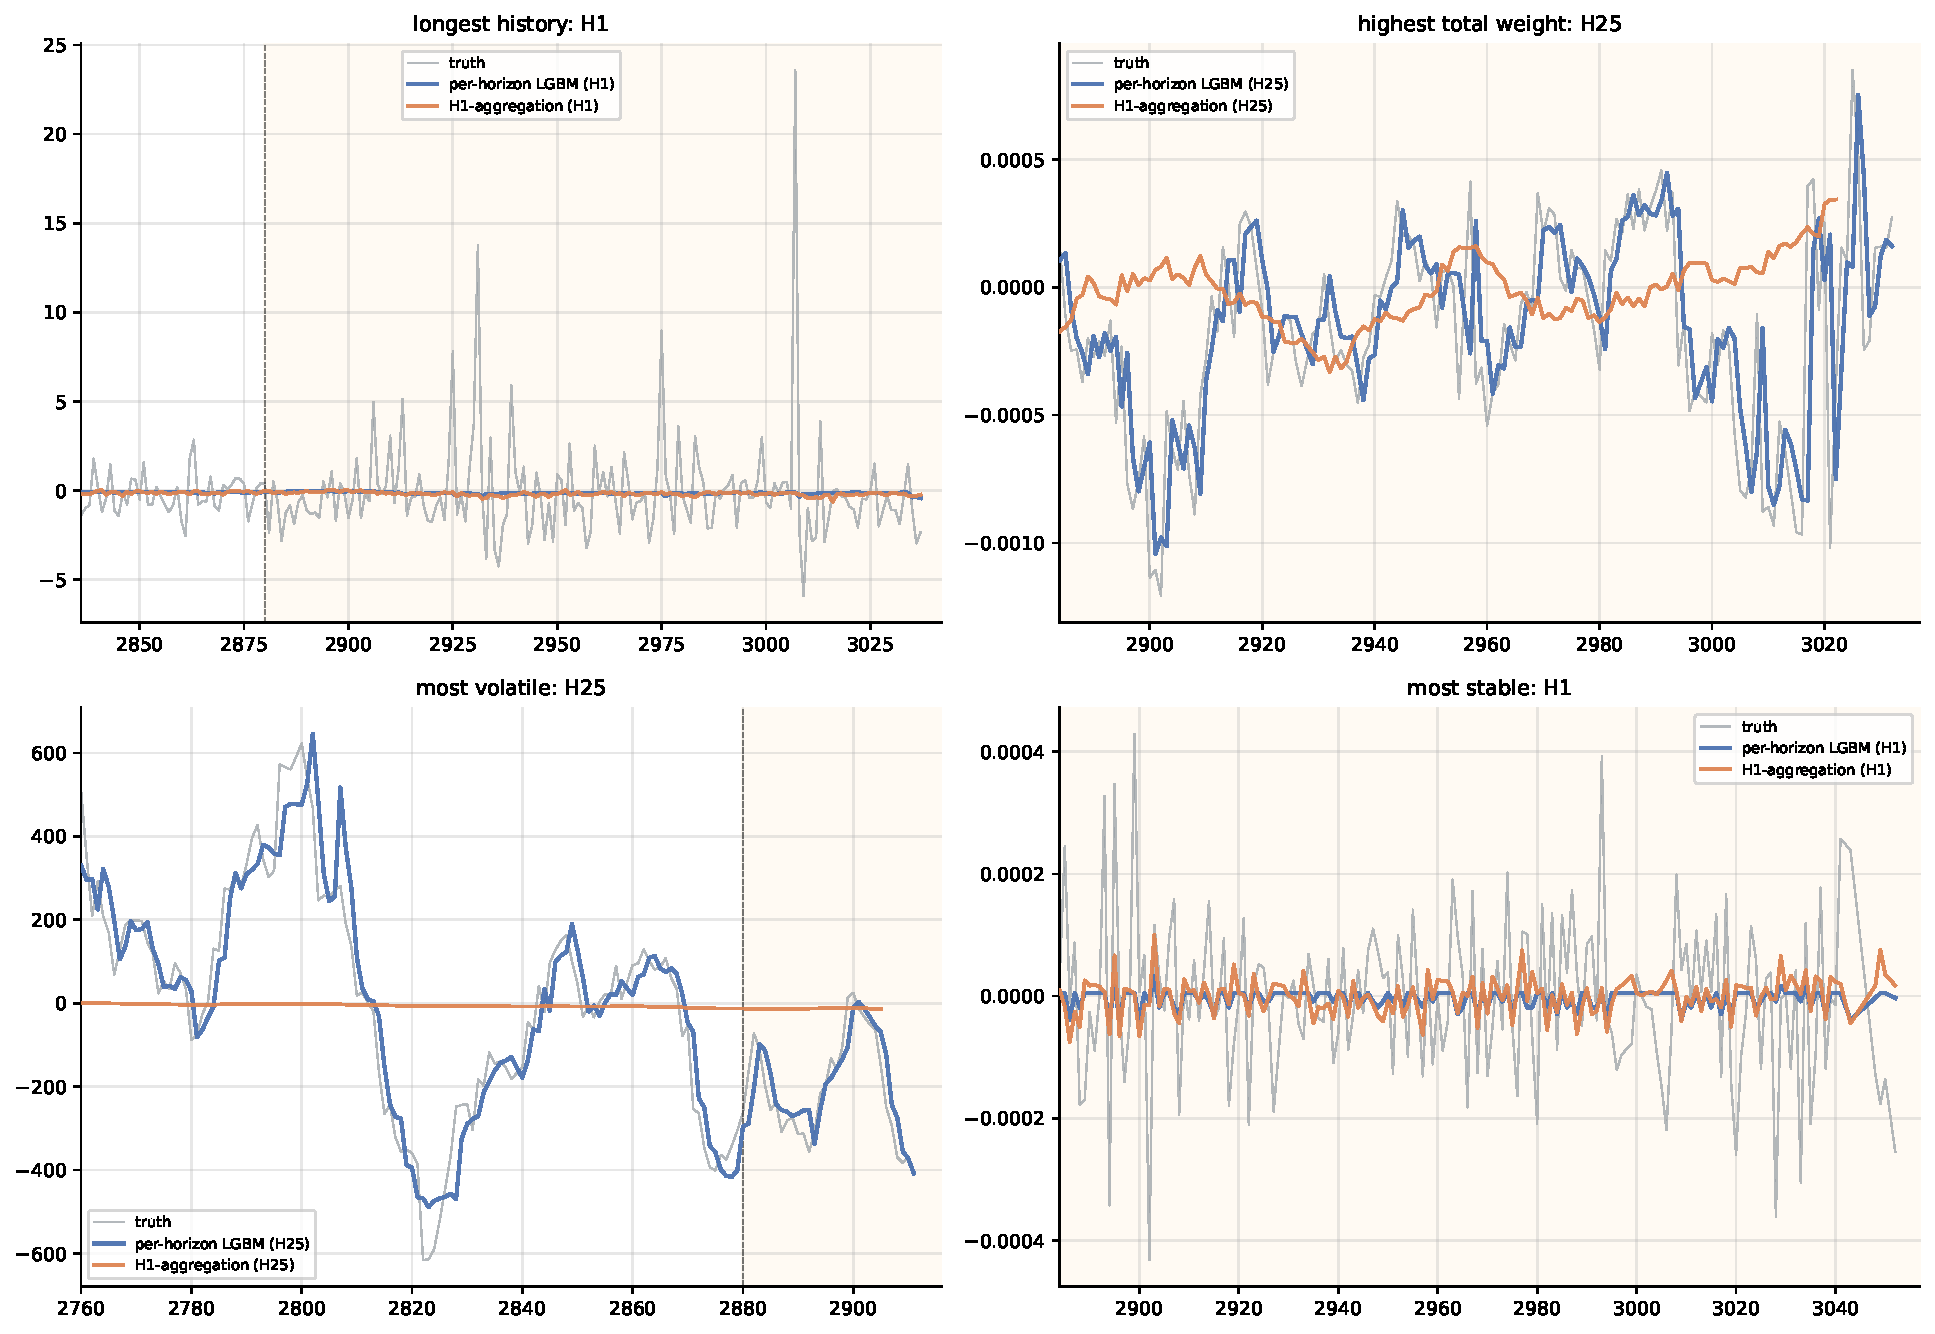
\includegraphics[width=\linewidth]{04_h1_aggregation_overlay_4series}
\caption{Forecast overlays on the four representative series at their native horizons. Truth in muted grey, per-horizon LightGBM in blue, H1-aggregation in orange. The orange line stays close to zero on every panel, while the blue line tracks the truth where signal is available.}
\label{fig:h1_agg_overlay}
\end{figure}

\subsection{Research gap identified}
\label{sec:analysis:research_gap}

The H1-aggregation experiment identifies a concrete methodological gap that the project has not closed. The cumulation property is structurally exploitable in principle but only by a model whose H1 predictions are accurate enough that the aggregated noise stays below the H$k$ signal magnitude. Three avenues are open for future work:

\begin{enumerate}
  \item \textbf{Stronger H1 model.} A more capacity-rich H1 model --- larger LightGBM, deeper recurrent network with feature inputs, gradient-boosted-quantile regressor for asymmetric loss --- might increase the H1 model's standalone skill enough that aggregated predictions stay below the H$k$ target's magnitude. The bound is set by the cumulation correlation: even a perfect H1 predictor would only recover an aggregated H25 skill of about $0.91$ before clipping.
  \item \textbf{Joint multi-task model.} Rather than choosing between per-horizon-independent and H1-only architectures, train a single multi-output LightGBM (or deep model) that predicts all four horizons simultaneously and is regularised toward the cumulation constraint $\hat y^{H_k}_t \approx \sum_i \hat y^{H_1}_{t+i}$ as a soft loss. This combines the per-horizon model's direct fit on cumulative targets with the cumulation strategy's structural consistency.
  \item \textbf{Hybrid scaling.} Apply the H1-aggregation as a residual correction on top of the per-horizon model: predict H$k$ directly, then adjust by adding a calibrated multiple of $\sum \hat y^{H_1}$. This preserves the per-horizon model's signal while using the cumulation property to reduce variance on rows where it agrees with the direct prediction.
\end{enumerate}

The third option is the most modest and the most likely to produce a real improvement on this panel; it is the natural follow-up after the chapter's negative result.

\subsection{Headline empirical findings of the project so far}
\label{sec:analysis:headline}

Bringing the numerical results together:

\begin{itemize}
  \item \textbf{Global LightGBM on H3} achieves weighted skill $0.664$ on the canonical holdout (CI $[0.657, 0.671]$), beating the Naive floor of $0.464$ by $+0.20$ on the metric-decisive horizon (\cref{sec:lgbm}).
  \item \textbf{Per-horizon LightGBM} dominates across all four horizons, with marginal but statistically significant lifts over Naive at H10 and H25 because the cumulation property makes the long-horizon Naive itself a strong baseline.
  \item \textbf{The H1-aggregation strategy fails completely}: aggregating H1 predictions does not recover H$k$ predictions when the H1 model is signal-poor, because shrinkage toward zero compounds across the rolling sum. This is an unambiguous negative finding from a well-designed experiment, and it identifies a research gap that future work could close with a stronger H1 model or a joint multi-output architecture.
  \item \textbf{Probabilistic forecasting via quantile regression and split conformal calibration} (\cref{sec:quantile}) provides calibrated 80\% prediction intervals on the four representative series. The median LightGBM achieves point skill $0.83$ on the most-volatile series and $0.61$ on the highest-weight series; the calibrated intervals hit the nominal coverage target within bootstrap noise on three of four series.
\end{itemize}

\section{Converting the Forecast into Actions}
\label{sec:actions}

A weighted skill score above the naive floor is only useful if the forecast can be turned into an action that produces value at the scale of the weight on each row. This section sketches how a hedge-fund operator would translate the per-horizon predictions produced in \cref{sec:lgbm} into deployable position decisions.

\subsection{Weight as economic significance}

The competition \texttt{weight} column is plausibly a proxy for assets under management, notional traded size, or a similar measure of how much economic significance a particular row carries. In any of those interpretations, two operational consequences follow. First, the model's accuracy on the small set of high-weight rows determines how much capital the strategy can profitably deploy. Second, an action plan has to scale per-row position size by the local confidence in the forecast --- not just the point estimate.

\subsection{From point forecast to position size}

A simple deployable rule is to scale the absolute position taken on row $i$ proportionally to the predicted target sign and to the model's confidence on that row. Under a quadratic-utility approximation, the optimal position is
\[
  \pi_i \;\propto\; \frac{\hat y_i}{\sigma_i^2},
\]
where $\hat y_i$ is the point forecast and $\sigma_i$ is the predicted forecast uncertainty on the same row. The point forecast comes from the LightGBM model in \cref{sec:lgbm}; the uncertainty $\sigma_i$ is exactly what the probabilistic forecasting work scheduled for a later notebook will provide via quantile regression and split conformal calibration.

\subsection{Risk controls}

In practice, a deployment would also need:
\begin{itemize}
  \item \emph{Hard position limits} per series and per code, so a single high-weight row cannot dominate the portfolio.
  \item \emph{Coverage monitoring} on the conformal prediction intervals, so the operator can detect distribution drift between the training panel and live data.
  \item \emph{H3 tracking}, since H3 is the metric-decisive horizon (\cref{sec:weight_per_horizon}); H3-specific live skill should be a top-line dashboard metric.
\end{itemize}

This chapter will be expanded with the conformal-interval implementation and a worked numerical example after the probabilistic forecasting notebook lands.

\section{Future Work}
\label{sec:future_work}

Several extensions would meaningfully strengthen the project beyond the current scope:

\begin{enumerate}
  \item \textbf{Multi-horizon aggregation experiment.} Operationalise the cumulation hypothesis in \cref{sec:cumulation} by training a single LightGBM on the H=1 process and deriving H3, H10, H25 forecasts by rolling sum. Compare to the per-horizon-independent fits in \cref{sec:lgbm}.
  \item \textbf{Probabilistic forecasting via quantile regression and split conformal calibration.} Replace point forecasts with calibrated 80\% prediction intervals on every series. The legacy code in \texttt{Finial\_notebooks/04\_quantile\_regression\_codex.ipynb} provides a starting point; tighter integration with the canonical evaluation slice and bootstrap intervals on PICP coverage are the natural extensions.
  \item \textbf{Ensembles with leak-resistant fitting.} Fit weighted averages, ridge-stacking models, and per-series/per-horizon selection rules on the meta slice $\mathtt{ts\_index} \in (2880, 3240]$, score on the canonical holdout. The meta slice was reserved untouched across every chapter precisely so this experiment can be done without leakage.
  \item \textbf{Feature-aware deep models beyond recurrent architectures.} Test temporal convolutional networks (TCN) and small MLP-on-features variants under the same protocol used in \cref{sec:deep}. The expectation is that on this signal-poor panel the gain over feature-aware GRU is modest, but the comparison would close out the deep section.
  \item \textbf{Hyperparameter tuning depth.} The Optuna sweep in \cref{sec:lgbm} used 20 trials per horizon on a 200{,}000-row subsample. Extending to 50--100 trials per horizon on the full panel might add a small skill increment, especially on H3.
  \item \textbf{Cross-series transfer.} The 86 anonymised features and the cross-series correlations in \cref{sec:eda:cross_series} suggest there is shared structure across sub-codes within a code. A multi-task model that predicts all four horizons simultaneously, sharing a learned representation across sub-codes, could exploit this in a way the current per-horizon LightGBM does not.
\end{enumerate}

\section{References}
\label{sec:references}

\textit{Bibliography to be expanded with full BibTeX entries.} The methodology developed in this report draws on the following primary references:

\begin{enumerate}
  \item Box, G.~E.~P.\ and Jenkins, G.~M., \emph{Time Series Analysis: Forecasting and Control}, Holden-Day, 1970. The canonical reference for the AR / MA / ARMA / ARIMA family used in \cref{sec:classical}.
  \item Dickey, D.~A.\ and Fuller, W.~A., ``Distribution of the Estimators for Autoregressive Time Series with a Unit Root'', \emph{Journal of the American Statistical Association}, 74(366a):427--431, 1979. Augmented Dickey--Fuller test, used in \cref{sec:eda:stationarity}.
  \item Kwiatkowski, D.\ et al., ``Testing the Null Hypothesis of Stationarity Against the Alternative of a Unit Root'', \emph{Journal of Econometrics}, 54(1--3):159--178, 1992. KPSS test, used in \cref{sec:eda:stationarity}.
  \item Cleveland, R.~B.\ et al., ``STL: A Seasonal-Trend Decomposition Procedure Based on Loess'', \emph{Journal of Official Statistics}, 6(1):3--73, 1990. STL decomposition used in \cref{sec:eda:stl}.
  \item Akaike, H., ``A New Look at the Statistical Model Identification'', \emph{IEEE Transactions on Automatic Control}, 19(6):716--723, 1974. Akaike Information Criterion, with the small-sample-corrected variant of \cite{burnham_anderson} used for model selection in \cref{sec:classical:lineup}.
  \item Ke, G.\ et al., ``LightGBM: A Highly Efficient Gradient Boosting Decision Tree'', \emph{NeurIPS} 2017. The gradient-boosted regressor used in \cref{sec:lgbm}.
  \item Akiba, T.\ et al., ``Optuna: A Next-generation Hyperparameter Optimization Framework'', \emph{KDD} 2019. The Bayesian hyperparameter sweep used in \cref{sec:lgbm:tuning}.
  \item Hochreiter, S.\ and Schmidhuber, J., ``Long Short-Term Memory'', \emph{Neural Computation}, 9(8):1735--1780, 1997. LSTM architecture used in \cref{sec:deep}.
  \item Cho, K.\ et al., ``Learning Phrase Representations Using RNN Encoder-Decoder for Statistical Machine Translation'', \emph{EMNLP} 2014. GRU architecture used in \cref{sec:deep}.
  \item Vovk, V., Gammerman, A.\ and Shafer, G., \emph{Algorithmic Learning in a Random World}, Springer, 2005. Conformal prediction framework, scheduled for the probabilistic forecasting chapter.
  \item Romano, Y., Patterson, E.\ and Cand\`es, E., ``Conformalized Quantile Regression'', \emph{NeurIPS} 2019. CQR construction used in the probabilistic forecasting chapter.
  \item Burnham, K.~P.\ and Anderson, D.~R., \emph{Model Selection and Multimodel Inference}, Springer, 2002. Recommends AICc whenever $n / k < 40$.
\end{enumerate}

Additional references on the Kaggle competition page itself, the polars dataframe library, statsmodels, MAPIE, and PyTorch will be added in the final pass.


\end{document}
